% Options for packages loaded elsewhere
\PassOptionsToPackage{unicode}{hyperref}
\PassOptionsToPackage{hyphens}{url}
\PassOptionsToPackage{dvipsnames,svgnames*,x11names*}{xcolor}
%
\documentclass[
  12pt,
]{article}
\usepackage{lmodern}
\usepackage{setspace}
\usepackage{amssymb,amsmath}
\usepackage{ifxetex,ifluatex}
\ifnum 0\ifxetex 1\fi\ifluatex 1\fi=0 % if pdftex
  \usepackage[T1]{fontenc}
  \usepackage[utf8]{inputenc}
  \usepackage{textcomp} % provide euro and other symbols
\else % if luatex or xetex
  \usepackage{unicode-math}
  \defaultfontfeatures{Scale=MatchLowercase}
  \defaultfontfeatures[\rmfamily]{Ligatures=TeX,Scale=1}
  \setmainfont[]{Times New Roman}
  \setsansfont[]{Times New Roman}
\fi
% Use upquote if available, for straight quotes in verbatim environments
\IfFileExists{upquote.sty}{\usepackage{upquote}}{}
\IfFileExists{microtype.sty}{% use microtype if available
  \usepackage[]{microtype}
  \UseMicrotypeSet[protrusion]{basicmath} % disable protrusion for tt fonts
}{}
\makeatletter
\@ifundefined{KOMAClassName}{% if non-KOMA class
  \IfFileExists{parskip.sty}{%
    \usepackage{parskip}
  }{% else
    \setlength{\parindent}{0pt}
    \setlength{\parskip}{6pt plus 2pt minus 1pt}}
}{% if KOMA class
  \KOMAoptions{parskip=half}}
\makeatother
\usepackage{xcolor}
\IfFileExists{xurl.sty}{\usepackage{xurl}}{} % add URL line breaks if available
\IfFileExists{bookmark.sty}{\usepackage{bookmark}}{\usepackage{hyperref}}
\hypersetup{
  colorlinks=true,
  linkcolor=Maroon,
  filecolor=Maroon,
  citecolor=Blue,
  urlcolor=Blue,
  pdfcreator={LaTeX via pandoc}}
\urlstyle{same} % disable monospaced font for URLs
\usepackage[margin=1in]{geometry}
\usepackage{color}
\usepackage{fancyvrb}
\newcommand{\VerbBar}{|}
\newcommand{\VERB}{\Verb[commandchars=\\\{\}]}
\DefineVerbatimEnvironment{Highlighting}{Verbatim}{commandchars=\\\{\}}
% Add ',fontsize=\small' for more characters per line
\usepackage{framed}
\definecolor{shadecolor}{RGB}{248,248,248}
\newenvironment{Shaded}{\begin{snugshade}}{\end{snugshade}}
\newcommand{\AlertTok}[1]{\textcolor[rgb]{0.94,0.16,0.16}{#1}}
\newcommand{\AnnotationTok}[1]{\textcolor[rgb]{0.56,0.35,0.01}{\textbf{\textit{#1}}}}
\newcommand{\AttributeTok}[1]{\textcolor[rgb]{0.77,0.63,0.00}{#1}}
\newcommand{\BaseNTok}[1]{\textcolor[rgb]{0.00,0.00,0.81}{#1}}
\newcommand{\BuiltInTok}[1]{#1}
\newcommand{\CharTok}[1]{\textcolor[rgb]{0.31,0.60,0.02}{#1}}
\newcommand{\CommentTok}[1]{\textcolor[rgb]{0.56,0.35,0.01}{\textit{#1}}}
\newcommand{\CommentVarTok}[1]{\textcolor[rgb]{0.56,0.35,0.01}{\textbf{\textit{#1}}}}
\newcommand{\ConstantTok}[1]{\textcolor[rgb]{0.00,0.00,0.00}{#1}}
\newcommand{\ControlFlowTok}[1]{\textcolor[rgb]{0.13,0.29,0.53}{\textbf{#1}}}
\newcommand{\DataTypeTok}[1]{\textcolor[rgb]{0.13,0.29,0.53}{#1}}
\newcommand{\DecValTok}[1]{\textcolor[rgb]{0.00,0.00,0.81}{#1}}
\newcommand{\DocumentationTok}[1]{\textcolor[rgb]{0.56,0.35,0.01}{\textbf{\textit{#1}}}}
\newcommand{\ErrorTok}[1]{\textcolor[rgb]{0.64,0.00,0.00}{\textbf{#1}}}
\newcommand{\ExtensionTok}[1]{#1}
\newcommand{\FloatTok}[1]{\textcolor[rgb]{0.00,0.00,0.81}{#1}}
\newcommand{\FunctionTok}[1]{\textcolor[rgb]{0.00,0.00,0.00}{#1}}
\newcommand{\ImportTok}[1]{#1}
\newcommand{\InformationTok}[1]{\textcolor[rgb]{0.56,0.35,0.01}{\textbf{\textit{#1}}}}
\newcommand{\KeywordTok}[1]{\textcolor[rgb]{0.13,0.29,0.53}{\textbf{#1}}}
\newcommand{\NormalTok}[1]{#1}
\newcommand{\OperatorTok}[1]{\textcolor[rgb]{0.81,0.36,0.00}{\textbf{#1}}}
\newcommand{\OtherTok}[1]{\textcolor[rgb]{0.56,0.35,0.01}{#1}}
\newcommand{\PreprocessorTok}[1]{\textcolor[rgb]{0.56,0.35,0.01}{\textit{#1}}}
\newcommand{\RegionMarkerTok}[1]{#1}
\newcommand{\SpecialCharTok}[1]{\textcolor[rgb]{0.00,0.00,0.00}{#1}}
\newcommand{\SpecialStringTok}[1]{\textcolor[rgb]{0.31,0.60,0.02}{#1}}
\newcommand{\StringTok}[1]{\textcolor[rgb]{0.31,0.60,0.02}{#1}}
\newcommand{\VariableTok}[1]{\textcolor[rgb]{0.00,0.00,0.00}{#1}}
\newcommand{\VerbatimStringTok}[1]{\textcolor[rgb]{0.31,0.60,0.02}{#1}}
\newcommand{\WarningTok}[1]{\textcolor[rgb]{0.56,0.35,0.01}{\textbf{\textit{#1}}}}
\usepackage{longtable,booktabs}
% Correct order of tables after \paragraph or \subparagraph
\usepackage{etoolbox}
\makeatletter
\patchcmd\longtable{\par}{\if@noskipsec\mbox{}\fi\par}{}{}
\makeatother
% Allow footnotes in longtable head/foot
\IfFileExists{footnotehyper.sty}{\usepackage{footnotehyper}}{\usepackage{footnote}}
\makesavenoteenv{longtable}
\usepackage{graphicx,grffile}
\makeatletter
\def\maxwidth{\ifdim\Gin@nat@width>\linewidth\linewidth\else\Gin@nat@width\fi}
\def\maxheight{\ifdim\Gin@nat@height>\textheight\textheight\else\Gin@nat@height\fi}
\makeatother
% Scale images if necessary, so that they will not overflow the page
% margins by default, and it is still possible to overwrite the defaults
% using explicit options in \includegraphics[width, height, ...]{}
\setkeys{Gin}{width=\maxwidth,height=\maxheight,keepaspectratio}
% Set default figure placement to htbp
\makeatletter
\def\fps@figure{htbp}
\makeatother
\setlength{\emergencystretch}{3em} % prevent overfull lines
\providecommand{\tightlist}{%
  \setlength{\itemsep}{0pt}\setlength{\parskip}{0pt}}
\setcounter{secnumdepth}{5}
\usepackage{dcolumn}
\usepackage{color}
\usepackage{pdfpages}
\usepackage{booktabs}
\usepackage{longtable}
\usepackage{array}
\usepackage{multirow}
\usepackage{wrapfig}
\usepackage{float}
\usepackage{colortbl}
\usepackage{pdflscape}
\usepackage{tabu}
\usepackage{threeparttable}
\usepackage{threeparttablex}
\usepackage[normalem]{ulem}
\usepackage{makecell}
\usepackage{xcolor}

\title{\vspace{1cm}Literate programming with Python, R, Julia and Stata*\footnote{*Corresponding address: \href{mailto:miguel.portela@eeg.uminho.pt}{\nolinkurl{miguel.portela@eeg.uminho.pt}}.}\vspace{0.5cm}\\}
\author{Miguel Portela\\
~\\
Minho University\\}
\date{16 December, 2019\\
~\\}

\begin{document}
\maketitle
\begin{abstract}
\noindent\setstretch{1}In this presentation I will discuss how we can enhance the workflow by using literate programming to combine key features of different statistical packages, namely Stata, R, Julia and Python, on the one hand, and Latex as the typesetting system on the other. The goal is to demonstrate and share a template aiming at producing a highly automated report, or research paper, within the same framework. The tasks will run from exploratory data analysis to regression analysis, where the output, from summary to regression tables and figures, is seamlessly included in the final document. Furthermore, important elements of Latex editing, such as automatic referencing, will be highlighted. We aim at freeing the researcher form repetitive tasks to focus on critical and creative writing. Efficiency and replicability will be at the core of the discussion. RStudio will be used to edit and compile R Markdown. The focus will be on producing PDF outputs. In the presentation I will make use of packages such as bookdown, knitr, stargazer, dlookr, ggplot2, plotly, Statamarkdown, reticulate, JuliaCall, pandas, numpy, matplotlib or FixedEffectModels. The current code is an adaptation of the Rmd by Paul C. Bauer, Mannheim Centre for European Social Research, \href{mailto:mail@paulcbauer.eu}{\nolinkurl{mail@paulcbauer.eu}}..\vspace{.8cm}
\end{abstract}

\setstretch{1.2}
\clearpage

\renewcommand{\baselinestretch}{0.5}\normalsize

\renewcommand{\baselinestretch}{1.1}\normalsize

\clearpage

\hypertarget{exploratory-data-analysis}{%
\section{Exploratory data analysis}\label{exploratory-data-analysis}}

I start by exploring the data \textbf{NLSWORK} (National Longitudinal Survey. Young Women 14-26 years of age in 1968).

\begin{Shaded}
\begin{Highlighting}[]
\CommentTok{## ExPanDaR: Explore Panel Data Interactively}

  \KeywordTok{library}\NormalTok{(ExPanDaR)}
    
    \CommentTok{## type ExPanD() in the Console}

\KeywordTok{setwd}\NormalTok{(}\StringTok{"/Users/miguelportela/Documents/GitHub/prjs/logs"}\NormalTok{)}

\KeywordTok{library}\NormalTok{(haven)}
\KeywordTok{library}\NormalTok{(ggplot2)}

\NormalTok{nlswork <-}\StringTok{ }\KeywordTok{read_dta}\NormalTok{(}\StringTok{"/Users/miguelportela/Documents/GitHub/prjs/data/nlswork.dta"}\NormalTok{)}

\NormalTok{nls<-}\KeywordTok{data.frame}\NormalTok{(nlswork)}

\KeywordTok{attach}\NormalTok{(nlswork)}

\KeywordTok{head}\NormalTok{(nlswork)}
\end{Highlighting}
\end{Shaded}

\hypertarget{a-tibble-6-x-21}{%
\section{A tibble: 6 x 21}\label{a-tibble-6-x-21}}

idcode year birth\_yr age race msp nev\_mar grade collgrad not\_smsa
\textless dbl+l\textgreater{}
1 1 70 51 18 2 {[}bla\textasciitilde{} 0 1 12 0 0
2 1 71 51 19 2 {[}bla\textasciitilde{} 1 0 12 0 0
3 1 72 51 20 2 {[}bla\textasciitilde{} 1 0 12 0 0
4 1 73 51 21 2 {[}bla\textasciitilde{} 1 0 12 0 0
5 1 75 51 23 2 {[}bla\textasciitilde{} 1 0 12 0 0
6 1 77 51 25 2 {[}bla\textasciitilde{} 0 0 12 0 0
\# \ldots{} with 11 more variables: c\_city , south , ind\_code ,
\# occ\_code , union , wks\_ue , ttl\_exp , tenure ,
\# hours , wks\_work , ln\_wage

\begin{Shaded}
\begin{Highlighting}[]
\KeywordTok{library}\NormalTok{(stargazer)}
\KeywordTok{stargazer}\NormalTok{(nls, }
          \DataTypeTok{title =} \StringTok{"Summary statistics"}\NormalTok{,}
          \DataTypeTok{label=}\StringTok{"tab1"}\NormalTok{, }
          \DataTypeTok{table.placement =} \StringTok{"ht"}\NormalTok{, }
          \DataTypeTok{header=}\OtherTok{FALSE}\NormalTok{)}
\end{Highlighting}
\end{Shaded}

\begin{table}[ht] \centering 
  \caption{Summary statistics} 
  \label{tab1} 
\begin{tabular}{@{\extracolsep{5pt}}lccccccc} 
\\[-1.8ex]\hline 
\hline \\[-1.8ex] 
Statistic & \multicolumn{1}{c}{N} & \multicolumn{1}{c}{Mean} & \multicolumn{1}{c}{St. Dev.} & \multicolumn{1}{c}{Min} & \multicolumn{1}{c}{Pctl(25)} & \multicolumn{1}{c}{Pctl(75)} & \multicolumn{1}{c}{Max} \\ 
\hline \\[-1.8ex] 
idcode & 28,534 & 2,601.284 & 1,487.359 & 1 & 1,327 & 3,881 & 5,159 \\ 
year & 28,534 & 77.959 & 6.384 & 68 & 72 & 83 & 88 \\ 
birth\_yr & 28,534 & 48.085 & 3.013 & 41 & 46 & 51 & 54 \\ 
age & 28,510 & 29.045 & 6.701 & 14.000 & 23.000 & 34.000 & 46.000 \\ 
race & 28,534 & 1.303 & 0.482 & 1 & 1 & 2 & 3 \\ 
msp & 28,518 & 0.603 & 0.489 & 0.000 & 0.000 & 1.000 & 1.000 \\ 
nev\_mar & 28,518 & 0.230 & 0.421 & 0.000 & 0.000 & 0.000 & 1.000 \\ 
grade & 28,532 & 12.533 & 2.324 & 0.000 & 12.000 & 14.000 & 18.000 \\ 
collgrad & 28,534 & 0.168 & 0.374 & 0 & 0 & 0 & 1 \\ 
not\_smsa & 28,526 & 0.282 & 0.450 & 0.000 & 0.000 & 1.000 & 1.000 \\ 
c\_city & 28,526 & 0.357 & 0.479 & 0.000 & 0.000 & 1.000 & 1.000 \\ 
south & 28,526 & 0.410 & 0.492 & 0.000 & 0.000 & 1.000 & 1.000 \\ 
ind\_code & 28,193 & 7.693 & 2.994 & 1.000 & 5.000 & 11.000 & 12.000 \\ 
occ\_code & 28,413 & 4.778 & 3.065 & 1.000 & 3.000 & 6.000 & 13.000 \\ 
union & 19,238 & 0.234 & 0.424 & 0.000 & 0.000 & 0.000 & 1.000 \\ 
wks\_ue & 22,830 & 2.548 & 7.294 & 0.000 & 0.000 & 0.000 & 76.000 \\ 
ttl\_exp & 28,534 & 6.215 & 4.652 & 0.000 & 2.462 & 9.128 & 28.885 \\ 
tenure & 28,101 & 3.124 & 3.751 & 0.000 & 0.500 & 4.167 & 25.917 \\ 
hours & 28,467 & 36.560 & 9.870 & 1.000 & 35.000 & 40.000 & 168.000 \\ 
wks\_work & 27,831 & 53.989 & 29.032 & 0.000 & 36.000 & 72.000 & 104.000 \\ 
ln\_wage & 28,534 & 1.675 & 0.478 & 0.000 & 1.361 & 1.964 & 5.264 \\ 
\hline \\[-1.8ex] 
\end{tabular} 
\end{table}

\begin{verbatim}
 [1] "idcode"   "year"     "birth_yr" "age"      "race"     "msp"     
 [7] "nev_mar"  "grade"    "collgrad" "not_smsa" "c_city"   "south"   
[13] "ind_code" "occ_code" "union"    "wks_ue"   "ttl_exp"  "tenure"  
[19] "hours"    "wks_work" "ln_wage" 
\end{verbatim}

\includegraphics{rmarkdown_report_files/figure-latex/unnamed-chunk-4-1.pdf} \includegraphics{rmarkdown_report_files/figure-latex/unnamed-chunk-4-2.pdf} \includegraphics{rmarkdown_report_files/figure-latex/unnamed-chunk-4-3.pdf}

\begin{verbatim}
 num [1:28534] 1.45 1.03 1.59 1.78 1.78 ...
 - attr(*, "label")= chr "ln(wage/GNP deflator)"
 - attr(*, "format.stata")= chr "%9.0g"
\end{verbatim}

\includegraphics{rmarkdown_report_files/figure-latex/unnamed-chunk-4-4.pdf} \includegraphics{rmarkdown_report_files/figure-latex/unnamed-chunk-4-5.pdf} \includegraphics{rmarkdown_report_files/figure-latex/unnamed-chunk-4-6.pdf} \includegraphics{rmarkdown_report_files/figure-latex/unnamed-chunk-4-7.pdf}

The average age in our data is 29.

\hypertarget{sec:tables}{%
\section{Tables}\label{sec:tables}}

Producing good tables and referencing these tables within a R Markdown PDF has been a hassle but got much better. Examples that you may use are shown below. The way you reference tables is slightly different, e.g., for \texttt{stargazer} the label is contained in the function, for \texttt{kable} it's contained in the chunk name.

\hypertarget{stargazer-summary-and-regression-tables}{%
\subsection{stargazer(): Summary and regression tables}\label{stargazer-summary-and-regression-tables}}

Table \ref{tab1} shows summary stats of your data.\footnote{To reference the table where you set the identifier in the stargazer function you only need to use the actual label, i.e., ´tab1´.} I normally use \texttt{stargazer()} (Hlavac \protect\hyperlink{ref-hlavac2013stargazer}{2013}) which offers extreme flexibility regarding table output (see \texttt{?stargazer}).

\begin{Shaded}
\begin{Highlighting}[]
\KeywordTok{library}\NormalTok{(stargazer)}
\KeywordTok{stargazer}\NormalTok{(cars, }
          \DataTypeTok{title =} \StringTok{"Summary table with stargazer"}\NormalTok{,}
          \DataTypeTok{label=}\StringTok{"tab1cars"}\NormalTok{, }
          \DataTypeTok{table.placement =} \StringTok{"H"}\NormalTok{, }
          \DataTypeTok{header=}\OtherTok{FALSE}\NormalTok{)}
\end{Highlighting}
\end{Shaded}

\begin{table}[H] \centering 
  \caption{Summary table with stargazer} 
  \label{tab1cars} 
\begin{tabular}{@{\extracolsep{5pt}}lccccccc} 
\\[-1.8ex]\hline 
\hline \\[-1.8ex] 
Statistic & \multicolumn{1}{c}{N} & \multicolumn{1}{c}{Mean} & \multicolumn{1}{c}{St. Dev.} & \multicolumn{1}{c}{Min} & \multicolumn{1}{c}{Pctl(25)} & \multicolumn{1}{c}{Pctl(75)} & \multicolumn{1}{c}{Max} \\ 
\hline \\[-1.8ex] 
speed & 50 & 15.400 & 5.288 & 4 & 12 & 19 & 25 \\ 
dist & 50 & 42.980 & 25.769 & 2 & 26 & 56 & 120 \\ 
\hline \\[-1.8ex] 
\end{tabular} 
\end{table}

Table \ref{tab2} shows the output for a regression table. Make sure you name all your models and explicitly refer to model names (M1, M2 etc.) in the text.

\begin{Shaded}
\begin{Highlighting}[]
\KeywordTok{library}\NormalTok{(stargazer)}
\NormalTok{model1 <-}\StringTok{ }\KeywordTok{lm}\NormalTok{(speed }\OperatorTok{~}\StringTok{ }\NormalTok{dist, }\DataTypeTok{data =}\NormalTok{ cars)}
\NormalTok{model2 <-}\StringTok{ }\KeywordTok{lm}\NormalTok{(speed }\OperatorTok{~}\StringTok{ }\NormalTok{dist, }\DataTypeTok{data =}\NormalTok{ cars)}
\NormalTok{model3 <-}\StringTok{ }\KeywordTok{lm}\NormalTok{(dist }\OperatorTok{~}\StringTok{ }\NormalTok{speed, }\DataTypeTok{data =}\NormalTok{ cars)}
\KeywordTok{stargazer}\NormalTok{(model1, model2, model3,}
          \DataTypeTok{title =} \StringTok{"Regression table with stargazer"}\NormalTok{,}
          \DataTypeTok{label=}\StringTok{"tab2"}\NormalTok{, }
          \DataTypeTok{table.placement =} \StringTok{"H"}\NormalTok{, }
          \DataTypeTok{column.labels =} \KeywordTok{c}\NormalTok{(}\StringTok{"M1"}\NormalTok{, }\StringTok{"M2"}\NormalTok{, }\StringTok{"M3"}\NormalTok{),}
          \DataTypeTok{model.numbers =} \OtherTok{FALSE}\NormalTok{,}
          \DataTypeTok{header=}\OtherTok{FALSE}\NormalTok{)}
\end{Highlighting}
\end{Shaded}

\begin{table}[H] \centering 
  \caption{Regression table with stargazer} 
  \label{tab2} 
\begin{tabular}{@{\extracolsep{5pt}}lccc} 
\\[-1.8ex]\hline 
\hline \\[-1.8ex] 
 & \multicolumn{3}{c}{\textit{Dependent variable:}} \\ 
\cline{2-4} 
\\[-1.8ex] & \multicolumn{2}{c}{speed} & dist \\ 
 & M1 & M2 & M3 \\ 
\hline \\[-1.8ex] 
 dist & 0.166$^{***}$ & 0.166$^{***}$ &  \\ 
  & (0.017) & (0.017) &  \\ 
  & & & \\ 
 speed &  &  & 3.932$^{***}$ \\ 
  &  &  & (0.416) \\ 
  & & & \\ 
 Constant & 8.284$^{***}$ & 8.284$^{***}$ & $-$17.579$^{**}$ \\ 
  & (0.874) & (0.874) & (6.758) \\ 
  & & & \\ 
\hline \\[-1.8ex] 
Observations & 50 & 50 & 50 \\ 
R$^{2}$ & 0.651 & 0.651 & 0.651 \\ 
Adjusted R$^{2}$ & 0.644 & 0.644 & 0.644 \\ 
Residual Std. Error (df = 48) & 3.156 & 3.156 & 15.380 \\ 
F Statistic (df = 1; 48) & 89.567$^{***}$ & 89.567$^{***}$ & 89.567$^{***}$ \\ 
\hline 
\hline \\[-1.8ex] 
\textit{Note:}  & \multicolumn{3}{r}{$^{*}$p$<$0.1; $^{**}$p$<$0.05; $^{***}$p$<$0.01} \\ 
\end{tabular} 
\end{table}

\hypertarget{figures}{%
\section{Figures}\label{figures}}

\hypertarget{r-base-graphs}{%
\subsection{R base graphs}\label{r-base-graphs}}

Inserting figures can be slightly more complicated. Ideally, we would produce and insert them directly in the \texttt{.rmd} file. It's relatively simple to insert R base graphs as you can see in Figure \ref{fig:fig-1}.

\begin{Shaded}
\begin{Highlighting}[]
\KeywordTok{plot}\NormalTok{(cars}\OperatorTok{$}\NormalTok{speed, cars}\OperatorTok{$}\NormalTok{dist)}
\end{Highlighting}
\end{Shaded}

\begin{figure}[H]

{\centering \includegraphics{rmarkdown_report_files/figure-latex/fig-1-1} 

}

\caption{Scatterplot of Speed and Distance}\label{fig:fig-1}
\end{figure}

But it turns out that it doesn't always work so well.

\hypertarget{ggplot2-graphs}{%
\subsection{ggplot2 graphs}\label{ggplot2-graphs}}

Same is true for ggplot2 as you can see in Figure \ref{fig:fig-2}.

\begin{Shaded}
\begin{Highlighting}[]
\NormalTok{mtcars}\OperatorTok{$}\NormalTok{cyl <-}\StringTok{ }\KeywordTok{as.factor}\NormalTok{(mtcars}\OperatorTok{$}\NormalTok{cyl) }\CommentTok{# Convert cyl to factor}
\KeywordTok{library}\NormalTok{(ggplot2)}
\KeywordTok{ggplot}\NormalTok{(mtcars, }\KeywordTok{aes}\NormalTok{(}\DataTypeTok{x=}\NormalTok{wt, }\DataTypeTok{y=}\NormalTok{mpg, }\DataTypeTok{shape=}\NormalTok{cyl)) }\OperatorTok{+}\StringTok{ }\KeywordTok{geom_point}\NormalTok{() }\OperatorTok{+}
\StringTok{  }\KeywordTok{labs}\NormalTok{(}\DataTypeTok{x=}\StringTok{"Weight (lb/1000)"}\NormalTok{, }\DataTypeTok{y =} \StringTok{"Miles/(US) gallon"}\NormalTok{, }
       \DataTypeTok{shape=}\StringTok{"Number of }\CharTok{\textbackslash{}n}\StringTok{ Cylinders"}\NormalTok{) }\OperatorTok{+}\StringTok{ }\KeywordTok{theme_classic}\NormalTok{()}
\end{Highlighting}
\end{Shaded}

\begin{figure}[H]

{\centering \includegraphics{rmarkdown_report_files/figure-latex/fig-2-1} 

}

\caption{Miles per gallon according to the weight}\label{fig:fig-2}
\end{figure}

\hypertarget{plotly-graphs}{%
\subsection{Plotly graphs}\label{plotly-graphs}}

Plotly is a popular graph engine that let's you also produce interactive graphs that you can embed in html webpages or documents (e.g., see \href{https://paulcbauer.shinyapps.io/visualizing-causal-scenarios/}{here}). I am a big fan. For some time there was no easy, automatic way to insert high resolution Plotly graphs into your R Markdown PDF. However, this changed since Plotly provided Orca, a command line application for generating static images from Plotly graphs. The installation is a bit tricky (see here: \url{https://github.com/plotly/orca\#installation}) but once you get it running you can produce beautiful graphs and include them in your RMarkdown PDF using some simple latex as shown below in Figure \ref{fig:fig-3}. Potentially, in case you did not install the command line application this part may fail. If so simply exclude the chunk and the latex code.

\begin{Shaded}
\begin{Highlighting}[]
\KeywordTok{library}\NormalTok{(plotly)}
\NormalTok{p <-}\StringTok{ }\KeywordTok{plot_ly}\NormalTok{(cars, }\DataTypeTok{type =} \StringTok{"scatter"}\NormalTok{, }\DataTypeTok{mode=}\StringTok{"markers"}\NormalTok{,}
        \DataTypeTok{x=}\OperatorTok{~}\NormalTok{speed, }
        \DataTypeTok{y=}\OperatorTok{~}\NormalTok{dist)}
\KeywordTok{Sys.setenv}\NormalTok{(}\StringTok{'MAPBOX_TOKEN'}\NormalTok{ =}\StringTok{ '12423423'}\NormalTok{) }\CommentTok{# set arbitrary token}
\KeywordTok{orca}\NormalTok{(p, }\StringTok{"plotly-plot.pdf"}\NormalTok{)}
\end{Highlighting}
\end{Shaded}

\begin{figure}[ht]
\centering
\caption{An plotly plot that was exported as PDF with orca before}\label{fig:fig-3}
        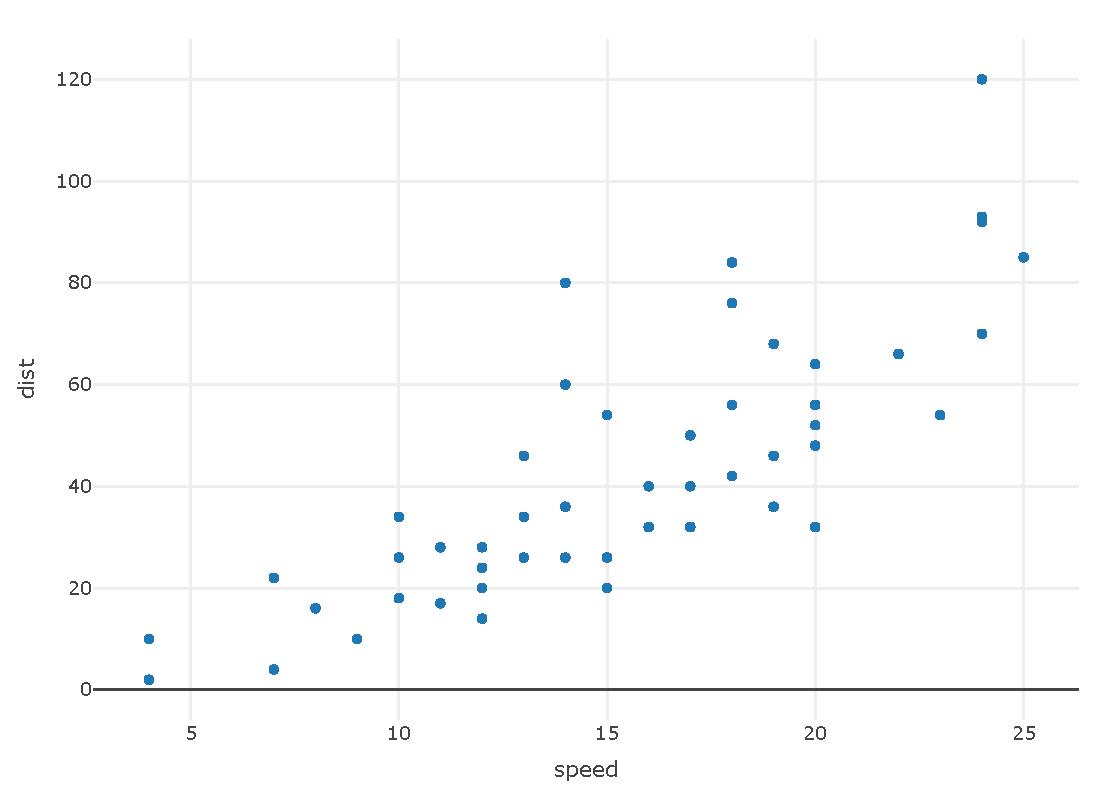
\includegraphics[width=0.9\linewidth]{plotly-plot.pdf}
\begin{flushleft}
\end{flushleft}
\end{figure}
\vspace{-1.2cm}

\hypertarget{python}{%
\section{Python}\label{python}}

\hypertarget{api-data-download-using-python}{%
\subsection{API data download using Python}\label{api-data-download-using-python}}

\begin{Shaded}
\begin{Highlighting}[]
\ImportTok{import}\NormalTok{ sys}
\BuiltInTok{print}\NormalTok{(sys.version)}
\end{Highlighting}
\end{Shaded}

\begin{verbatim}
3.8.0 (v3.8.0:fa919fdf25, Oct 14 2019, 10:23:27) 
[Clang 6.0 (clang-600.0.57)]
\end{verbatim}

\begin{Shaded}
\begin{Highlighting}[]
\ImportTok{import}\NormalTok{ json}
\CommentTok{##from json.decoder import JSONDecodeError}
\ImportTok{import}\NormalTok{ requests}
\ImportTok{import}\NormalTok{ numpy }\ImportTok{as}\NormalTok{ np}
\ImportTok{import}\NormalTok{ pandas }\ImportTok{as}\NormalTok{ pd}

\CommentTok{## INE: https://www.ine.pt/ine/json_indicador/pindica.jsp?}
\CommentTok{## op=2&varcd=0008074&Dim1=S7A2015&Dim2=200&Dim3=3&lang=PT}

\CommentTok{# api-endpoint }

\NormalTok{URL }\OperatorTok{=} \StringTok{"https://www.ine.pt/ine/json_indicador/pindica.jsp"}
  
\CommentTok{# define parameters}

\NormalTok{OP}\OperatorTok{=}\StringTok{"2"}
\NormalTok{VARCD}\OperatorTok{=}\StringTok{"0008074"}
\NormalTok{DIM1}\OperatorTok{=}\StringTok{"S7A2015"}
\NormalTok{DIM2}\OperatorTok{=}\StringTok{"200"}
\NormalTok{DIM3}\OperatorTok{=}\StringTok{"3"}
\NormalTok{LANG}\OperatorTok{=}\StringTok{"PT"}


\CommentTok{# defining a params dict for the parameters to be sent to the API }
\NormalTok{PARAMS }\OperatorTok{=}\NormalTok{ \{}\StringTok{'op'}\NormalTok{:OP,}\StringTok{'varcd'}\NormalTok{:VARCD,}\StringTok{'Dim1'}\NormalTok{:DIM1,}\StringTok{'Dim2'}\NormalTok{:DIM2,}\StringTok{'Dim3'}\NormalTok{:DIM3,}\StringTok{'lang'}\NormalTok{:LANG\} }
  
\CommentTok{# sending get request and saving the response as response object }
\NormalTok{r }\OperatorTok{=}\NormalTok{ requests.get(url }\OperatorTok{=}\NormalTok{ URL,params}\OperatorTok{=}\NormalTok{PARAMS) }
  
\CommentTok{# extracting data in json format }
\NormalTok{data }\OperatorTok{=}\NormalTok{ r.json() }

\NormalTok{valor }\OperatorTok{=}\NormalTok{ data[}\DecValTok{0}\NormalTok{][}\StringTok{'Dados'}\NormalTok{][}\StringTok{'2015'}\NormalTok{][}\DecValTok{0}\NormalTok{][}\StringTok{'valor'}\NormalTok{]}

\NormalTok{valor}
\end{Highlighting}
\end{Shaded}

\begin{verbatim}
'1.8'
\end{verbatim}

The value is 1.8.

This works fine and as expected.

\begin{Shaded}
\begin{Highlighting}[]
\NormalTok{x }\OperatorTok{=} \DecValTok{42} \OperatorTok{*} \DecValTok{2}
\BuiltInTok{print}\NormalTok{(x) }
\end{Highlighting}
\end{Shaded}

\begin{verbatim}
84
\end{verbatim}

The value of \texttt{x} in the Python session is 84.

\hypertarget{import-data-from-pdf-files}{%
\subsection{Import data from PDF files}\label{import-data-from-pdf-files}}

\begin{Shaded}
\begin{Highlighting}[]
  \BuiltInTok{cd}\NormalTok{ /Users/miguelportela/Documents/GitHub/prjs/pdfs}
    \FunctionTok{find}\NormalTok{ . -name }\StringTok{'*.pdf'}\NormalTok{ -print0 }\KeywordTok{|} \FunctionTok{xargs}\NormalTok{ -0 -n1 pdfsandwich -gray}
    \FunctionTok{find}\NormalTok{ . -name }\StringTok{'*ocr.pdf'}\NormalTok{ -print0 }\KeywordTok{|} \FunctionTok{xargs}\NormalTok{ -0 -n1 pdftotext}
\end{Highlighting}
\end{Shaded}

\begin{verbatim}
['', 'PORTARIAS 111111111 DE REGULAMENTAGAO DO TRABALHO', 'PORTARIAs de EXTENSAO 444444444', 'PE das alteragdes do CCT entre a aa tt Assoc e a Feder x32PORTARIAs de EXTENSAO 444444444', '', '', 'Marmores e Materiais de Construcado 222222222', '', '', 'PE das alteragdes do CCT entre a aa tt Assoc e a Feder x32PORTARIAs de EXTENSAO 444444444']
   
FILE:  sample_text_v4
match 1
match 4
match 1
match 4
match 1
match 4
match 3
match 1
match 4
['zzzz', 'PE dasalteragoes do, CCTentre a Assoc. Nacional  dos, Opticos e a FETESE -- Feder. dos Sind. dos Trabalhadores', 'XXXXXXXX', 'akjshdkjashjkds', 'askjhdkjsahkjd']
   
FILE:  sample_text_v5
-> match 5
PE dasalteragoes do, CCTentre a Assoc. Nacional  dos, Opticos e a FETESE -- Feder. dos Sind. dos Trabalhadores
99999
\end{verbatim}

\begin{verbatim}
   linha  ...          source
0      1  ...  sample_text_v4
1      2  ...  sample_text_v4
2      3  ...  sample_text_v4
3      6  ...  sample_text_v4
4      9  ...  sample_text_v4
5      1  ...  sample_text_v5

[6 rows x 4 columns]
\end{verbatim}

And now we use Stata to explore the data.

\begin{Shaded}
\begin{Highlighting}[]

\NormalTok{quiet cd }\StringTok{"/Users/miguelportela/Documents/GitHub/prjs/logs"}
\NormalTok{quiet import delimited }\StringTok{"/Users/miguelportela/Documents/GitHub/prjs/data/PE.csv"}\NormalTok{, encoding(ISO-8859-2) }\KeywordTok{clear} 
\KeywordTok{tab}\NormalTok{ source}
\end{Highlighting}
\end{Shaded}

\begin{verbatim}
 command window is unrecognized
r(199);

        source |      Freq.     Percent        Cum.
---------------+-----------------------------------
sample_text_v4 |          5       83.33       83.33
sample_text_v5 |          1       16.67      100.00
---------------+-----------------------------------
         Total |          6      100.00
\end{verbatim}

\begin{Shaded}
\begin{Highlighting}[]

\KeywordTok{quietly}\NormalTok{\{}
\NormalTok{cd /Users/miguelportela/Documents/GitHub/prjs/chunks}

\KeywordTok{use}\NormalTok{ nipcs, }\KeywordTok{clear}
\KeywordTok{compress}
\KeywordTok{contract}\NormalTok{ nipc}
\KeywordTok{drop}\NormalTok{ _freq}
\KeywordTok{drop} \KeywordTok{if}\NormalTok{ nipc == .}
\KeywordTok{format}\NormalTok{ %12.0f nipc}
\NormalTok{\}}

\KeywordTok{codebook}\NormalTok{ nipc}

\KeywordTok{tab}\NormalTok{ nipc}
\end{Highlighting}
\end{Shaded}

\begin{verbatim}
 command window is unrecognized
r(199);




-------------------------------------------------------------------------------
nipc                                                                (unlabeled)
-------------------------------------------------------------------------------

                  type:  numeric (long)

                 range:  [5.106e+08,5.155e+08]        units:  1
         unique values:  23                       missing .:  0/23

                  mean:   5.1e+08
              std. dev:   1.9e+06

           percentiles:        10%       25%       50%       75%       90%

       nipc |      Freq.     Percent        Cum.
------------+-----------------------------------
  510649068 |          1        4.35        4.35
  510779174 |          1        4.35        8.70
  511056737 |          1        4.35       13.04
  511117060 |          1        4.35       17.39
  511124899 |          1        4.35       21.74
  511240619 |          1        4.35       26.09
  511247478 |          1        4.35       30.43
  513208348 |          1        4.35       34.78
  513587128 |          1        4.35       39.13
  514118890 |          1        4.35       43.48
  514525657 |          1        4.35       47.83
  514532718 |          1        4.35       52.17
  514591889 |          1        4.35       56.52
  515002666 |          1        4.35       60.87
  515080985 |          1        4.35       65.22
  515092550 |          1        4.35       69.57
  515092649 |          1        4.35       73.91
  515464236 |          1        4.35       78.26
  515478377 |          1        4.35       82.61
  515484920 |          1        4.35       86.96
  515517135 |          1        4.35       91.30
  515518565 |          1        4.35       95.65
  515522988 |          1        4.35      100.00
------------+-----------------------------------
      Total |         23      100.00
\end{verbatim}

\hypertarget{julia-experiments}{%
\section{Julia experiments}\label{julia-experiments}}

\hypertarget{computations}{%
\subsection{Computations}\label{computations}}

\begin{verbatim}
1.4142135623730951
\end{verbatim}

\hypertarget{grab-results-in-r}{%
\subsection{Grab results in R}\label{grab-results-in-r}}

\begin{verbatim}
[1] 1.414214
\end{verbatim}

\begin{verbatim}
Julia Object of type FixedEffectModel.
                           Fixed Effect Model                           
=========================================================================
Number of obs:               147715   Degrees of freedom:           67180
R2:                           0.978   R2 Adjusted:                  0.960
F Statistic:                 23.362   p-value:                      0.000
R2 within:                    0.001   Iterations:                     419
Converged:                     true   
=========================================================================
             Estimate   Std.Error t value Pr(>|t|)   Lower 95%  Upper 95%
-------------------------------------------------------------------------
education  0.00155631 0.000597587 2.60432    0.009 0.000385043 0.00272758
lnsales    0.00622989 0.000987569 6.30831    0.000  0.00429426 0.00816552
=========================================================================
\end{verbatim}

\begin{Shaded}
\begin{Highlighting}[]
\KeywordTok{use}\NormalTok{ /Users/miguelportela/Documents/GitHub/prjs/}\KeywordTok{data}\NormalTok{/data_short, }\KeywordTok{clear}

\KeywordTok{timer} \KeywordTok{on}\NormalTok{ 1}

\NormalTok{    reghdfe lnrealwage education lnsales,absorb(workerid firmid }\FunctionTok{year}\NormalTok{)}

\KeywordTok{timer} \KeywordTok{off}\NormalTok{ 1}
\KeywordTok{timer} \OtherTok{list}\NormalTok{ 1}
\KeywordTok{timer} \KeywordTok{clear}\NormalTok{ 1}
\end{Highlighting}
\end{Shaded}

\begin{verbatim}
 command window is unrecognized
r(199);


( )


(MWFE estimator converged in 236 iterations)

HDFE Linear regression                            Number of obs   =    147,715
Absorbing 3 HDFE groups                           F(   2,  99667) =      28.91
                                                  Prob > F        =     0.0000
                                                  R-squared       =     0.9782
                                                  Adj R-squared   =     0.9677
                                                  Within R-sq.    =     0.0006
                                                  Root MSE        =     0.0943

------------------------------------------------------------------------------
  lnrealwage |      Coef.   Std. Err.      t    P>|t|     [95% Conf. Interval]
-------------+----------------------------------------------------------------
   education |   .0015563   .0005372     2.90   0.004     .0005034    .0026092
     lnsales |   .0062299   .0008877     7.02   0.000     .0044899    .0079698
       _cons |   1.577908   .0148587   106.19   0.000     1.548785     1.60703
------------------------------------------------------------------------------

Absorbed degrees of freedom:
-----------------------------------------------------+
 Absorbed FE | Categories  - Redundant  = Num. Coefs |
-------------+---------------------------------------|
    workerid |     44047           0       44047     |
      firmid |     23127       19131        3996     |
        year |         4           1           3    ?|
-----------------------------------------------------+
? = number of redundant parameters may be higher


   1:     21.26 /        1 =      21.2590
\end{verbatim}

\begin{Shaded}
\begin{Highlighting}[]
\KeywordTok{library}\NormalTok{(lfe)}
\NormalTok{data_short <-}\StringTok{ }\KeywordTok{read_dta}\NormalTok{(}\StringTok{"/Users/miguelportela/Documents/GitHub/prjs/data/data_short.dta"}\NormalTok{)}

\KeywordTok{system.time}\NormalTok{(est_hdfe <-}\StringTok{ }\KeywordTok{felm}\NormalTok{(data_short}\OperatorTok{$}\NormalTok{lnrealwage }\OperatorTok{~}\StringTok{ }\NormalTok{data_short}\OperatorTok{$}\NormalTok{education }\OperatorTok{+}\StringTok{ }\NormalTok{data_short}\OperatorTok{$}\NormalTok{lnsales }\OperatorTok{|}\StringTok{ }\NormalTok{data_short}\OperatorTok{$}\NormalTok{workerid }\OperatorTok{+}\StringTok{ }\NormalTok{data_short}\OperatorTok{$}\NormalTok{firmid }\OperatorTok{+}\StringTok{ }\NormalTok{data_short}\OperatorTok{$}\NormalTok{year))}

\KeywordTok{summary}\NormalTok{(est_hdfe)}
\end{Highlighting}
\end{Shaded}

\vspace{0.3cm}

The estimated return to education is 0.2\%. The model has an \(R^2\) of 0.9782.

\hypertarget{output-julias-table-for-hdfe}{%
\subsection{Output Julia's table for HDFE}\label{output-julias-table-for-hdfe}}

\begin{table}[ht]
\label{tab:hdfe}
  \begin{tabular}{lrr}
\toprule
          & \multicolumn{2}{c}{lnrealwage} \\ 
\cmidrule(lr){2-3} 
          &      (1) &                 (2) \\ 
\midrule
education & 0.006*** &             0.002** \\ 
          &  (0.000) &             (0.001) \\ 
lnsales   & 0.013*** &            0.006*** \\ 
          &  (0.001) &             (0.001) \\ 
\midrule
workerid  &      Yes &                 Yes \\ 
year      &      Yes &                 Yes \\ 
firmid    &          &                 Yes \\ 
\midrule
Estimator &      OLS &                 OLS \\ 
\midrule
$N$       &  147,715 &             147,715 \\ 
$R^2$     &    0.970 &               0.978 \\ 
\bottomrule
\end{tabular}

\end{table}

\hypertarget{miguels-tests}{%
\section{Miguel's tests}\label{miguels-tests}}

\hypertarget{tasks}{%
\subsection{Tasks}\label{tasks}}

\emph{Produzir um relatório com base no NLSWORK, desde estatística descritiva, com os valores inseridos automaticamente no texto, gráficos e regressões. Com o Python corremos o EDA, Julia o REGHDFE for speed, com R o RMarkdown + functions \& Stata ??? functions???}

WORKSHOP: fazer uma acta do evento no formato de um `package' com a replicabilidade, markdown, \ldots{}

Python: explorar o Pandas e o Numpy

\hypertarget{r}{%
\subsection{R}\label{r}}

Table \ref{tab3} \ldots{} See Section \ref{sec:stata}

Example of an equation

\[\int_0^{2\pi} \sin x~dx\]

Example of a matrix

\[\mathbf{X} = \left[\begin{array}
{rrr}
1 & 2 & 3 \\
4 & 5 & 6 \\
7 & 8 & 9
\end{array}\right]
\]

\begin{equation}
f\left(k\right)=\binom{n}{k}p^k\left(1-p\right)^{n-k} \label{eq:binom}
\end{equation}

\$\$

See Equation \eqref{eq:binom}.

\begin{align}
y_{ijt} = \beta x_{ijt} + \eta_i + \gamma_j + \lambda_t + \varepsilon_{ijt}
\end{align}

\begin{table}[ht] \centering 
  \caption{Summary table} 
  \label{tab23} 
\begin{tabular}{@{\extracolsep{5pt}}lccc} 
\\[-1.8ex]\hline 
\hline \\[-1.8ex] 
Statistic & \multicolumn{1}{c}{N} & \multicolumn{1}{c}{Pctl(75)} & \multicolumn{1}{c}{St. Dev.} \\ 
\hline \\[-1.8ex] 
idcode & 28,534 & 3,881 & 1,487.359 \\ 
year & 28,534 & 83 & 6.384 \\ 
birth\_yr & 28,534 & 51 & 3.013 \\ 
age & 28,510 & 34.000 & 6.701 \\ 
race & 28,534 & 2 & 0.482 \\ 
msp & 28,518 & 1.000 & 0.489 \\ 
nev\_mar & 28,518 & 0.000 & 0.421 \\ 
grade & 28,532 & 14.000 & 2.324 \\ 
collgrad & 28,534 & 0 & 0.374 \\ 
not\_smsa & 28,526 & 1.000 & 0.450 \\ 
c\_city & 28,526 & 1.000 & 0.479 \\ 
south & 28,526 & 1.000 & 0.492 \\ 
ind\_code & 28,193 & 11.000 & 2.994 \\ 
occ\_code & 28,413 & 6.000 & 3.065 \\ 
union & 19,238 & 0.000 & 0.424 \\ 
wks\_ue & 22,830 & 0.000 & 7.294 \\ 
ttl\_exp & 28,534 & 9.128 & 4.652 \\ 
tenure & 28,101 & 4.167 & 3.751 \\ 
hours & 28,467 & 40.000 & 9.870 \\ 
wks\_work & 27,831 & 72.000 & 29.032 \\ 
ln\_wage & 28,534 & 1.964 & 0.478 \\ 
\hline \\[-1.8ex] 
\end{tabular} 
\end{table}

\begin{table}[ht] \centering 
  \caption{Regression table with stargazer} 
  \label{tab3} 
\begin{tabular}{@{\extracolsep{5pt}}lccc} 
\\[-1.8ex]\hline 
\hline \\[-1.8ex] 
 & \multicolumn{3}{c}{\textit{Dependent variable:}} \\ 
\cline{2-4} 
\\[-1.8ex] & \multicolumn{3}{c}{price} \\ 
 & M1 & M2 & M3 \\ 
\hline \\[-1.8ex] 
 mpg & $-$49.512 & $-$52.217 & $-$63.210 \\ 
  & (86.156) & (83.740) & (84.218) \\ 
  & & & \\ 
 weight & 1.747$^{***}$ & 2.111$^{***}$ & 2.442$^{***}$ \\ 
  & (0.641) & (0.619) & (0.688) \\ 
  & & & \\ 
 rep78 &  &  &  \\ 
  &  &  &  \\ 
  & & & \\ 
\hline \\[-1.8ex] 
Observations & 74 & 69 & 69 \\ 
R$^{2}$ & 0.293 & 0.365 & 0.376 \\ 
Adjusted R$^{2}$ & 0.273 & 0.335 & 0.337 \\ 
Residual Std. Error & 2,514.029 (df = 71) & 2,374.370 (df = 65) & 2,370.832 (df = 64) \\ 
F Statistic & 14.740$^{***}$ (df = 2; 71) & 12.437$^{***}$ (df = 3; 65) & 9.654$^{***}$ (df = 4; 64) \\ 
\hline 
\hline \\[-1.8ex] 
\textit{Note:}  & \multicolumn{3}{r}{$^{*}$p$<$0.1; $^{**}$p$<$0.05; $^{***}$p$<$0.01} \\ 
\end{tabular} 
\end{table}

\includegraphics{rmarkdown_report_files/figure-latex/unnamed-chunk-17-1.pdf}

\begin{Shaded}
\begin{Highlighting}[]
\KeywordTok{library}\NormalTok{(stargazer)}
\KeywordTok{stargazer}\NormalTok{(cars, }
          \DataTypeTok{title =} \StringTok{"Summary 24"}\NormalTok{,}
          \DataTypeTok{label=}\StringTok{"tab24"}\NormalTok{, }
          \DataTypeTok{table.placement =} \StringTok{"ht"}\NormalTok{, }
          \DataTypeTok{header=}\OtherTok{FALSE}\NormalTok{)}
\end{Highlighting}
\end{Shaded}

\begin{table}[ht] \centering 
  \caption{Summary 24} 
  \label{tab24} 
\begin{tabular}{@{\extracolsep{5pt}}lccccccc} 
\\[-1.8ex]\hline 
\hline \\[-1.8ex] 
Statistic & \multicolumn{1}{c}{N} & \multicolumn{1}{c}{Mean} & \multicolumn{1}{c}{St. Dev.} & \multicolumn{1}{c}{Min} & \multicolumn{1}{c}{Pctl(25)} & \multicolumn{1}{c}{Pctl(75)} & \multicolumn{1}{c}{Max} \\ 
\hline \\[-1.8ex] 
speed & 50 & 15.400 & 5.288 & 4 & 12 & 19 & 25 \\ 
dist & 50 & 42.980 & 25.769 & 2 & 26 & 56 & 120 \\ 
\hline \\[-1.8ex] 
\end{tabular} 
\end{table}

\hypertarget{sec:stata}{%
\subsection{Stata}\label{sec:stata}}

This a Stata example, Arellano (\protect\hyperlink{ref-arellano2003panel}{2003}). See also Arellano and Bond (\protect\hyperlink{ref-arellano1991some}{1991}) and Blundell and Bond (\protect\hyperlink{ref-bb98}{1998}). While \ldots{} (check Arellano and Bover \protect\hyperlink{ref-arellano1995another}{1995}).

\begin{verbatim}
 command window is unrecognized
r(199);

    Variable |        Obs        Mean    Std. Dev.       Min        Max
-------------+---------------------------------------------------------
       price |         74    6165.257    2949.496       3291      15906

     Repair |
Record 1978 |      Freq.     Percent        Cum.
------------+-----------------------------------
          1 |          2        2.90        2.90
          2 |          8       11.59       14.49
          3 |         30       43.48       57.97
          4 |         18       26.09       84.06
          5 |         11       15.94      100.00
------------+-----------------------------------
      Total |         69      100.00





(file /Users/miguelportela/Documents/GitHub/prjs/logs/density.pdf written in PD
> F format)

      Source |       SS           df       MS      Number of obs   =       234
-------------+----------------------------------   F(7, 226)       =     46.99
       Model |  145.879747         7  20.8399639   Prob > F        =    0.0000
    Residual |  100.230749       226  .443498888   R-squared       =    0.5927
-------------+----------------------------------   Adj R-squared   =    0.5801
       Total |  246.110496       233  1.05626822   Root MSE        =    .66596

------------------------------------------------------------------------------
       lngdp |      Coef.   Std. Err.      t    P>|t|     [95% Conf. Interval]
-------------+----------------------------------------------------------------
   education |   .2136664   .0193553    11.04   0.000     .1755265    .2518063
         lnk |   .1978085   .0308039     6.42   0.000     .1371089    .2585082
       openk |   .0062439   .0011852     5.27   0.000     .0039085    .0085794
             |
        year |
       1975  |  -.0694608   .1387178    -0.50   0.617    -.3428064    .2038849
       1980  |   -.177992   .1401702    -1.27   0.205    -.4541996    .0982156
       1985  |  -.2226975   .1400607    -1.59   0.113    -.4986894    .0532943
       1990  |    -.34965   .1425169    -2.45   0.015    -.6304819   -.0688182
             |
       _cons |    3.38917   .7508785     4.51   0.000     1.909552    4.868789
------------------------------------------------------------------------------
\end{verbatim}

The mean is \texttt{s\ \$xx} \ldots{}

\begin{figure}
\centering
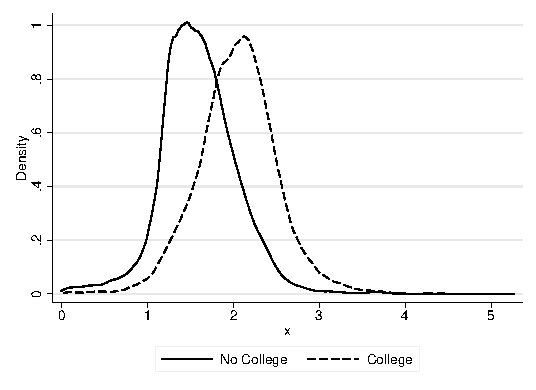
\includegraphics{logs/density.pdf}
\caption{Wage density}
\end{figure}

\begin{table}[ht]
\caption{Regression analysis}
\label{tab:stata}
  \begin{center}
\begin{tabular}{lccc}
\hline \noalign{\smallskip} & Simple model & Include capital & Full model\\
\noalign{\smallskip}\hline \noalign{\smallskip}Education & 0.3169*** & 0.212*** & 0.2***\\
 & \begin{footnotesize}(0.0093)\end{footnotesize} & \begin{footnotesize}(0.020)\end{footnotesize} & \begin{footnotesize}(0.0)\end{footnotesize}\\
\noalign{\smallskip}Capital &  & 0.125*** & 0.2***\\
 & \begin{footnotesize}\end{footnotesize} & \begin{footnotesize}(0.029)\end{footnotesize} & \begin{footnotesize}(0.0)\end{footnotesize}\\
\noalign{\smallskip}Openness degree &  &  & 0.0***\\
 & \begin{footnotesize}\end{footnotesize} & \begin{footnotesize}\end{footnotesize} & \begin{footnotesize}(0.0)\end{footnotesize}\\
\noalign{\smallskip}$R^2$ & 0.58 & 0.54 & 0.59\\
RMSE & 0.78 & 0.70 & 0.67\\
$N$ & 857 & 234 & 234\\
\noalign{\smallskip}\hline\end{tabular}\\
\smallskip\begin{footnotesize}\ * $p<0$.1; ** $p<0$.05; *** $p<0$.01\end{footnotesize}\\
\smallskip
\end{center}

\end{table}

We now export a set of statistics to an Excel file.

\begin{verbatim}
 command window is unrecognized
r(199);


version 15.1

/Users/miguelportela/Library/Application Support/Stata/ado/plus/x/xtabond2.ado

Checksum for /Users/miguelportela/Library/Application Support/Stata/ado/plus/x/
> xtabond2.ado = 616966544, size = 39434

/Users/miguelportela/Documents/GitHub/prjs/logs



Variable   Obs Unique      Mean       Min       Max  Label
-------------------------------------------------------------------------------
country    839    106         .         .         .  Country name
year       839      9  1980.906      1960      2000  Year of observation
education  839    574  4.794076       .04     12.25  Education
lngdp      839    838  9.308131  5.983335  12.51058  Log Real GDP per Worker
open       839      2  .4982122         0         1  1 = high degree of open...
gdp        839    838  20100.66  396.7612  271192.2  GDP level
-------------------------------------------------------------------------------


Note: file will be replaced when the first putexcel command is issued


`"a"' `"b"' `"c"' `"d"' `"e"' `"f"' `"g"' `"h"' `"i"' `"j"' `"k"' `"l"' `"m"' `
> "n"' `"p"' `"r"' `"s"' `"t"' `"u"' `"v"' `"z"'




Country's first letter:     a

    Insufficient number of countries; n countries = 5




Country's first letter:     b

    Number of countries:    11




Country's first letter:     c

    Number of countries:    9




Country's first letter:     d

    Insufficient number of countries; n countries = 2




Country's first letter:     e

    Insufficient number of countries; n countries = 5




Country's first letter:     f

    Insufficient number of countries; n countries = 3




Country's first letter:     g

    Insufficient number of countries; n countries = 4




Country's first letter:     h

    Insufficient number of countries; n countries = 4




Country's first letter:     i

    Number of countries:    7




Country's first letter:     j

    Insufficient number of countries; n countries = 3




Country's first letter:     k

    Insufficient number of countries; n countries = 2




Country's first letter:     l

    Insufficient number of countries; n countries = 2




Country's first letter:     m

    Number of countries:    8




Country's first letter:     n

    Number of countries:    6




Country's first letter:     p

    Number of countries:    7




Country's first letter:     r

    Insufficient number of countries; n countries = 2




Country's first letter:     s

    Number of countries:    14




Country's first letter:     t

    Insufficient number of countries; n countries = 5




Country's first letter:     u

    Insufficient number of countries; n countries = 4




Country's first letter:     v

    Insufficient number of countries; n countries = 1




Country's first letter:     z

    Insufficient number of countries; n countries = 2
\end{verbatim}

\begin{Shaded}
\begin{Highlighting}[]
\NormalTok{x =}\StringTok{ }\DecValTok{5}  \CommentTok{# radius of a circle}
\end{Highlighting}
\end{Shaded}

For a circle with the radius 5,
its area is 78.5398163.

See Figure \ref{fig:fig-tmp}.

\begin{figure}[ht]

{\centering \includegraphics{rmarkdown_report_files/figure-latex/fig-tmp-1} 

}

\caption{Scatterplot test MP}\label{fig:fig-tmp}
\end{figure}

\hypertarget{final-remarks}{%
\section{Final remarks}\label{final-remarks}}

Check: \url{https://github.com/tlamadon/blm-replicate}

\newpage

\hypertarget{appendix}{%
\section{Appendix}\label{appendix}}

\hypertarget{software-versioning}{%
\subsection{Software versioning}\label{software-versioning}}

\begin{Shaded}
\begin{Highlighting}[]
\KeywordTok{cat}\NormalTok{(}\KeywordTok{paste}\NormalTok{(}\StringTok{"#"}\NormalTok{, }\KeywordTok{capture.output}\NormalTok{(}\KeywordTok{sessionInfo}\NormalTok{()), }\StringTok{"}\CharTok{\textbackslash{}n}\StringTok{"}\NormalTok{, }\DataTypeTok{collapse =}\StringTok{""}\NormalTok{)) }
\end{Highlighting}
\end{Shaded}

\begin{verbatim}
# R version 3.6.1 (2019-07-05) 
# Platform: x86_64-apple-darwin15.6.0 (64-bit) 
# Running under: macOS Catalina 10.15.2 
#  
# Matrix products: default 
# BLAS:   /Library/Frameworks/R.framework/Versions/3.6/Resources/lib/libRblas.0.dylib 
# LAPACK: /Library/Frameworks/R.framework/Versions/3.6/Resources/lib/libRlapack.dylib 
#  
# locale: 
# [1] en_US.UTF-8/en_US.UTF-8/en_US.UTF-8/C/en_US.UTF-8/en_US.UTF-8 
#  
# attached base packages: 
# [1] stats     graphics  grDevices utils     datasets  methods   base      
#  
# other attached packages: 
#  [1] JuliaCall_0.17.1    plotly_4.9.1        naniar_0.4.2        
#  [4] visdat_0.5.3        dlookr_0.3.12       mice_3.6.0          
#  [7] lattice_0.20-38     dplyr_0.8.3         ggplot2_3.2.1       
# [10] haven_2.1.1         ExPanDaR_0.4.0      Statamarkdown_0.3.9 
# [13] stargazer_5.2.2     reticulate_1.13     
#  
# loaded via a namespace (and not attached): 
#   [1] readxl_1.3.1          backports_1.1.5       Hmisc_4.2-0           
#   [4] corrplot_0.84         plyr_1.8.4            lazyeval_0.2.2        
#   [7] splines_3.6.1         crosstalk_1.0.0       digest_0.6.20         
#  [10] htmltools_0.4.0       gdata_2.18.0          fansi_0.4.0           
#  [13] magrittr_1.5          checkmate_1.9.4       memoise_1.1.0         
#  [16] cluster_2.1.0         ROCR_1.0-7            openxlsx_4.1.0.1      
#  [19] readr_1.3.1           xts_0.11-2            sandwich_2.5-1        
#  [22] askpass_1.1           colorspace_1.4-1      blob_1.2.0            
#  [25] rvest_0.3.5           pan_1.6               xfun_0.11             
#  [28] tcltk_3.6.1           libcoin_1.0-5         crayon_1.3.4          
#  [31] jsonlite_1.6          lme4_1.1-21           zeallot_0.1.0         
#  [34] survival_2.44-1.1     zoo_1.8-6             glue_1.3.1            
#  [37] kableExtra_1.1.0      smbinning_0.9         gtable_0.3.0          
#  [40] UpSetR_1.4.0          webshot_0.5.1         car_3.0-4             
#  [43] quantmod_0.4-15       jomo_2.6-9            abind_1.4-5           
#  [46] scales_1.0.0          mvtnorm_1.0-11        DBI_1.0.0             
#  [49] Rcpp_1.0.3            viridisLite_0.3.0     xtable_1.8-4          
#  [52] htmlTable_1.13.2      foreign_0.8-72        bit_1.1-14            
#  [55] Formula_1.2-3         sqldf_0.4-11          DT_0.9                
#  [58] htmlwidgets_1.5.1     httr_1.4.1            gplots_3.0.1.1        
#  [61] RColorBrewer_1.1-2    acepack_1.4.1         ellipsis_0.3.0        
#  [64] pkgconfig_2.0.3       nnet_7.3-12           utf8_1.1.4            
#  [67] labeling_0.3          tidyselect_0.2.5      rlang_0.4.0           
#  [70] later_1.0.0           munsell_0.5.0         cellranger_1.1.0      
#  [73] tools_3.6.1           cli_1.1.0             gsubfn_0.7            
#  [76] generics_0.0.2        moments_0.14          RSQLite_2.1.2         
#  [79] broom_0.5.2           evaluate_0.14         stringr_1.4.0         
#  [82] fastmap_1.0.1         yaml_2.2.0            processx_3.4.1        
#  [85] knitr_1.26            bit64_0.9-7           shinycssloaders_0.2.0 
#  [88] zip_2.0.4             caTools_1.17.1.2      purrr_0.3.3           
#  [91] mitml_0.3-7           nlme_3.1-141          mime_0.7              
#  [94] tictoc_1.0            xml2_1.2.2            compiler_3.6.1        
#  [97] rstudioapi_0.10       curl_4.2              e1071_1.7-2           
# [100] tibble_2.1.3          stringi_1.4.3         ps_1.3.0              
# [103] forcats_0.4.0         Matrix_1.2-17         classInt_0.4-2        
# [106] nloptr_1.2.1          vctrs_0.2.0           RcmdrMisc_2.5-1       
# [109] pillar_1.4.2          lifecycle_0.1.0       data.table_1.12.6     
# [112] bitops_1.0-6          httpuv_1.5.2          R6_2.4.0              
# [115] latticeExtra_0.6-28   bookdown_0.16         promises_1.1.0        
# [118] KernSmooth_2.23-16    gridExtra_2.3         rio_0.5.16            
# [121] boot_1.3-23           MASS_7.3-51.4         gtools_3.8.1          
# [124] assertthat_0.2.1      chron_2.3-54          proto_1.0.0           
# [127] openssl_1.4.1         withr_2.1.2           nortest_1.0-4         
# [130] DMwR_0.4.1            parallel_3.6.1        hms_0.5.1             
# [133] grid_3.6.1            prettydoc_0.3.0       rpart_4.1-15          
# [136] tidyr_1.0.0           class_7.3-15          minqa_1.2.4           
# [139] inum_1.0-1            rmarkdown_2.0         carData_3.0-2         
# [142] TTR_0.23-5            partykit_1.2-5        shiny_1.4.0           
# [145] base64enc_0.1-3       tinytex_0.18          
\end{verbatim}

\begin{Shaded}
\begin{Highlighting}[]
  \CommentTok{# or use message() instead of cat()}
\end{Highlighting}
\end{Shaded}

\hypertarget{all-the-code-in-the-paper}{%
\subsection{All the code in the paper}\label{all-the-code-in-the-paper}}

To simply attach all the code you used in the PDF file in the appendix see the R chunk in the underlying \texttt{.rmd} file:

\begin{Shaded}
\begin{Highlighting}[]
\NormalTok{knitr}\OperatorTok{::}\NormalTok{opts_chunk}\OperatorTok{$}\KeywordTok{set}\NormalTok{(}\DataTypeTok{cache =} \OtherTok{FALSE}\NormalTok{)}
\CommentTok{# Use chache = TRUE if you want to speed up compilation}

\CommentTok{# A function to allow for showing some of the inline code}
\NormalTok{rinline <-}\StringTok{ }\ControlFlowTok{function}\NormalTok{(code)\{}
\NormalTok{  html <-}\StringTok{ '<code  class="r">``` `r CODE` ```</code>'}
  \KeywordTok{sub}\NormalTok{(}\StringTok{"CODE"}\NormalTok{, code, html)}

  \CommentTok{##https://opensource.com/article/19/5/python-3-default-mac}
  
  \KeywordTok{Sys.setenv}\NormalTok{(}\DataTypeTok{RETICULATE_PYTHON =} \StringTok{"/usr/local/bin/python3"}\NormalTok{)}
  
\CommentTok{##install.packages("reticulate")}
\KeywordTok{library}\NormalTok{(reticulate)}
\CommentTok{##use_python("/Library/Frameworks/Python.framework/Versions/3.8/bin/python3")}
  
\KeywordTok{use_virtualenv}\NormalTok{(}\StringTok{"/Users/miguelportela/.pyenv/version"}\NormalTok{)}
  
\CommentTok{##knitr::opts_chunk$set(python.reticulate=FALSE)}

\KeywordTok{library}\NormalTok{(JuliaCall)}

\KeywordTok{library}\NormalTok{(Statamarkdown)}
\NormalTok{stataexe <-}\StringTok{ "/Applications/Stata15/StataMP.app/Contents/MacOS//stata-mp"}
\NormalTok{knitr}\OperatorTok{::}\NormalTok{opts_chunk}\OperatorTok{$}\KeywordTok{set}\NormalTok{(}\DataTypeTok{engine.path=}\KeywordTok{list}\NormalTok{(}\DataTypeTok{stata=}\NormalTok{stataexe))}

\NormalTok{\}}
\KeywordTok{Sys.setenv}\NormalTok{(}\DataTypeTok{RETICULATE_PYTHON =} \StringTok{"/usr/local/bin/python3"}\NormalTok{)}
\KeywordTok{library}\NormalTok{(reticulate)}
\KeywordTok{use_virtualenv}\NormalTok{(}\StringTok{"/Users/miguelportela/.pyenv/version"}\NormalTok{)}
\KeywordTok{library}\NormalTok{(stargazer)}
\KeywordTok{library}\NormalTok{(Statamarkdown)}
\NormalTok{stataexe <-}\StringTok{ "/Applications/Stata15/StataMP.app/Contents/MacOS//stata-mp"}
\NormalTok{knitr}\OperatorTok{::}\NormalTok{opts_chunk}\OperatorTok{$}\KeywordTok{set}\NormalTok{(}\DataTypeTok{engine.path=}\KeywordTok{list}\NormalTok{(}\DataTypeTok{stata=}\NormalTok{stataexe))}


\CommentTok{## ExPanDaR: Explore Panel Data Interactively}

  \KeywordTok{library}\NormalTok{(ExPanDaR)}
    
    \CommentTok{## type ExPanD() in the Console}

\KeywordTok{setwd}\NormalTok{(}\StringTok{"/Users/miguelportela/Documents/GitHub/prjs/logs"}\NormalTok{)}

\KeywordTok{library}\NormalTok{(haven)}
\KeywordTok{library}\NormalTok{(ggplot2)}

\NormalTok{nlswork <-}\StringTok{ }\KeywordTok{read_dta}\NormalTok{(}\StringTok{"/Users/miguelportela/Documents/GitHub/prjs/data/nlswork.dta"}\NormalTok{)}

\NormalTok{nls<-}\KeywordTok{data.frame}\NormalTok{(nlswork)}

\KeywordTok{attach}\NormalTok{(nlswork)}

\KeywordTok{head}\NormalTok{(nlswork)}

\KeywordTok{library}\NormalTok{(stargazer)}
\KeywordTok{stargazer}\NormalTok{(nls, }
          \DataTypeTok{title =} \StringTok{"Summary statistics"}\NormalTok{,}
          \DataTypeTok{label=}\StringTok{"tab1"}\NormalTok{, }
          \DataTypeTok{table.placement =} \StringTok{"ht"}\NormalTok{, }
          \DataTypeTok{header=}\OtherTok{FALSE}\NormalTok{)}

\KeywordTok{library}\NormalTok{(dplyr)}
\KeywordTok{library}\NormalTok{(dlookr)}
\KeywordTok{library}\NormalTok{(ggplot2)}

\CommentTok{##eda_report(nlswork,output_dir = "/Users/miguelportela/Documents/GitHub/prjs/reports/",output_file = "eda_report.pdf")}

\CommentTok{## The data}

\KeywordTok{names}\NormalTok{(nlswork)}
\CommentTok{##summary(nlswork)}

\CommentTok{## Missing values}

\KeywordTok{library}\NormalTok{(}\StringTok{"visdat"}\NormalTok{)}

  \KeywordTok{vis_dat}\NormalTok{(nlswork)}

\CommentTok{## https://cran.r-project.org/web/packages/naniar/vignettes/naniar-visualisation.html}

\KeywordTok{library}\NormalTok{(naniar)}

  \KeywordTok{vis_miss}\NormalTok{(nlswork)}

  \KeywordTok{gg_miss_upset}\NormalTok{(nlswork)}

\CommentTok{## GRAPHS}
\NormalTok{dplyr}\OperatorTok{::}\KeywordTok{glimpse}\NormalTok{(nlswork}\OperatorTok{$}\NormalTok{ln_wage)}
\NormalTok{d <-}\StringTok{ }\KeywordTok{density}\NormalTok{(ln_wage)}
\KeywordTok{plot}\NormalTok{(d)}

\KeywordTok{plot}\NormalTok{(nls}\OperatorTok{$}\NormalTok{ln_wage,nls}\OperatorTok{$}\NormalTok{ttl_exp)}

\KeywordTok{ggplot}\NormalTok{(nlswork,}
       \KeywordTok{aes}\NormalTok{(}\DataTypeTok{x =}\NormalTok{ hours,}
           \DataTypeTok{y =}\NormalTok{ year)) }\OperatorTok{+}
\KeywordTok{geom_miss_point}\NormalTok{()}

\KeywordTok{ggplot}\NormalTok{(nlswork,}
       \KeywordTok{aes}\NormalTok{(}\DataTypeTok{x =}\NormalTok{ hours,}
           \DataTypeTok{y =}\NormalTok{ year)) }\OperatorTok{+}
\KeywordTok{geom_miss_point}\NormalTok{() }\OperatorTok{+}
\KeywordTok{facet_wrap}\NormalTok{(race)}

\NormalTok{stats <-}\StringTok{ }\KeywordTok{summary}\NormalTok{(nlswork}\OperatorTok{$}\NormalTok{age)}

\KeywordTok{library}\NormalTok{(stargazer)}
\KeywordTok{stargazer}\NormalTok{(cars, }
          \DataTypeTok{title =} \StringTok{"Summary table with stargazer"}\NormalTok{,}
          \DataTypeTok{label=}\StringTok{"tab1cars"}\NormalTok{, }
          \DataTypeTok{table.placement =} \StringTok{"H"}\NormalTok{, }
          \DataTypeTok{header=}\OtherTok{FALSE}\NormalTok{)}
\KeywordTok{library}\NormalTok{(stargazer)}
\NormalTok{model1 <-}\StringTok{ }\KeywordTok{lm}\NormalTok{(speed }\OperatorTok{~}\StringTok{ }\NormalTok{dist, }\DataTypeTok{data =}\NormalTok{ cars)}
\NormalTok{model2 <-}\StringTok{ }\KeywordTok{lm}\NormalTok{(speed }\OperatorTok{~}\StringTok{ }\NormalTok{dist, }\DataTypeTok{data =}\NormalTok{ cars)}
\NormalTok{model3 <-}\StringTok{ }\KeywordTok{lm}\NormalTok{(dist }\OperatorTok{~}\StringTok{ }\NormalTok{speed, }\DataTypeTok{data =}\NormalTok{ cars)}
\KeywordTok{stargazer}\NormalTok{(model1, model2, model3,}
          \DataTypeTok{title =} \StringTok{"Regression table with stargazer"}\NormalTok{,}
          \DataTypeTok{label=}\StringTok{"tab2"}\NormalTok{, }
          \DataTypeTok{table.placement =} \StringTok{"H"}\NormalTok{, }
          \DataTypeTok{column.labels =} \KeywordTok{c}\NormalTok{(}\StringTok{"M1"}\NormalTok{, }\StringTok{"M2"}\NormalTok{, }\StringTok{"M3"}\NormalTok{),}
          \DataTypeTok{model.numbers =} \OtherTok{FALSE}\NormalTok{,}
          \DataTypeTok{header=}\OtherTok{FALSE}\NormalTok{)}
\KeywordTok{plot}\NormalTok{(cars}\OperatorTok{$}\NormalTok{speed, cars}\OperatorTok{$}\NormalTok{dist)}
\NormalTok{mtcars}\OperatorTok{$}\NormalTok{cyl <-}\StringTok{ }\KeywordTok{as.factor}\NormalTok{(mtcars}\OperatorTok{$}\NormalTok{cyl) }\CommentTok{# Convert cyl to factor}
\KeywordTok{library}\NormalTok{(ggplot2)}
\KeywordTok{ggplot}\NormalTok{(mtcars, }\KeywordTok{aes}\NormalTok{(}\DataTypeTok{x=}\NormalTok{wt, }\DataTypeTok{y=}\NormalTok{mpg, }\DataTypeTok{shape=}\NormalTok{cyl)) }\OperatorTok{+}\StringTok{ }\KeywordTok{geom_point}\NormalTok{() }\OperatorTok{+}
\StringTok{  }\KeywordTok{labs}\NormalTok{(}\DataTypeTok{x=}\StringTok{"Weight (lb/1000)"}\NormalTok{, }\DataTypeTok{y =} \StringTok{"Miles/(US) gallon"}\NormalTok{, }
       \DataTypeTok{shape=}\StringTok{"Number of }\CharTok{\textbackslash{}n}\StringTok{ Cylinders"}\NormalTok{) }\OperatorTok{+}\StringTok{ }\KeywordTok{theme_classic}\NormalTok{()}
\KeywordTok{library}\NormalTok{(plotly)}
\NormalTok{p <-}\StringTok{ }\KeywordTok{plot_ly}\NormalTok{(cars, }\DataTypeTok{type =} \StringTok{"scatter"}\NormalTok{, }\DataTypeTok{mode=}\StringTok{"markers"}\NormalTok{,}
        \DataTypeTok{x=}\OperatorTok{~}\NormalTok{speed, }
        \DataTypeTok{y=}\OperatorTok{~}\NormalTok{dist)}
\KeywordTok{Sys.setenv}\NormalTok{(}\StringTok{'MAPBOX_TOKEN'}\NormalTok{ =}\StringTok{ '12423423'}\NormalTok{) }\CommentTok{# set arbitrary token}
\KeywordTok{orca}\NormalTok{(p, }\StringTok{"plotly-plot.pdf"}\NormalTok{)}
\NormalTok{import sys}
\KeywordTok{print}\NormalTok{(sys.version)}


\NormalTok{import json}
\CommentTok{##from json.decoder import JSONDecodeError}
\NormalTok{import requests}
\NormalTok{import numpy as np}
\NormalTok{import pandas as pd}

\CommentTok{## INE: https://www.ine.pt/ine/json_indicador/pindica.jsp?}
\CommentTok{## op=2&varcd=0008074&Dim1=S7A2015&Dim2=200&Dim3=3&lang=PT}

\CommentTok{# api-endpoint }

\NormalTok{URL =}\StringTok{ "https://www.ine.pt/ine/json_indicador/pindica.jsp"}
  
\CommentTok{# define parameters}

\NormalTok{OP=}\StringTok{"2"}
\NormalTok{VARCD=}\StringTok{"0008074"}
\NormalTok{DIM1=}\StringTok{"S7A2015"}
\NormalTok{DIM2=}\StringTok{"200"}
\NormalTok{DIM3=}\StringTok{"3"}
\NormalTok{LANG=}\StringTok{"PT"}


\CommentTok{# defining a params dict for the parameters to be sent to the API }
\NormalTok{PARAMS =}\StringTok{ }\NormalTok{\{}\StringTok{'op'}\OperatorTok{:}\NormalTok{OP,}\StringTok{'varcd'}\OperatorTok{:}\NormalTok{VARCD,}\StringTok{'Dim1'}\OperatorTok{:}\NormalTok{DIM1,}\StringTok{'Dim2'}\OperatorTok{:}\NormalTok{DIM2,}\StringTok{'Dim3'}\OperatorTok{:}\NormalTok{DIM3,}\StringTok{'lang'}\OperatorTok{:}\NormalTok{LANG\} }
  
\CommentTok{# sending get request and saving the response as response object }
\NormalTok{r =}\StringTok{ }\KeywordTok{requests.get}\NormalTok{(}\DataTypeTok{url =}\NormalTok{ URL,}\DataTypeTok{params=}\NormalTok{PARAMS) }
  
\CommentTok{# extracting data in json format }
\NormalTok{data =}\StringTok{ }\KeywordTok{r.json}\NormalTok{() }

\NormalTok{valor =}\StringTok{ }\NormalTok{data[}\DecValTok{0}\NormalTok{][}\StringTok{'Dados'}\NormalTok{][}\StringTok{'2015'}\NormalTok{][}\DecValTok{0}\NormalTok{][}\StringTok{'valor'}\NormalTok{]}

\NormalTok{valor}

\NormalTok{x =}\StringTok{ }\DecValTok{42} \OperatorTok{*}\StringTok{ }\DecValTok{2}
\KeywordTok{print}\NormalTok{(x) }
\NormalTok{  cd }\OperatorTok{/}\NormalTok{Users}\OperatorTok{/}\NormalTok{miguelportela}\OperatorTok{/}\NormalTok{Documents}\OperatorTok{/}\NormalTok{GitHub}\OperatorTok{/}\NormalTok{prjs}\OperatorTok{/}\NormalTok{pdfs}
\NormalTok{    find . }\OperatorTok{-}\NormalTok{name }\StringTok{'*.pdf'} \OperatorTok{-}\NormalTok{print0 }\OperatorTok{|}\StringTok{ }\NormalTok{xargs }\DecValTok{-0} \OperatorTok{-}\NormalTok{n1 pdfsandwich }\OperatorTok{-}\NormalTok{gray}
\NormalTok{    find . }\OperatorTok{-}\NormalTok{name }\StringTok{'*ocr.pdf'} \OperatorTok{-}\NormalTok{print0 }\OperatorTok{|}\StringTok{ }\NormalTok{xargs }\DecValTok{-0} \OperatorTok{-}\NormalTok{n1 pdftotext}
\NormalTok{import os}
\NormalTok{import numpy as np}
\NormalTok{import pandas as pd}
\NormalTok{import re}

\CommentTok{## CHECK PyPDF2}

\CommentTok{## wget -A pdf -m -p -E -k -K -np https://joram.madeira.gov.pt/joram/4serie/}
\CommentTok{## find . -name '*.pdf' -print0 | xargs -0 -n1 pdfsandwich -gray}
\CommentTok{## find . -name '*ocr.pdf' -print0 | xargs -0 -n1 pdftotext}

\CommentTok{# Create list with .txt files for the specified folder}
\NormalTok{files_list =}\StringTok{ }\KeywordTok{list}\NormalTok{()}
\ControlFlowTok{for}\NormalTok{ (dirpath, dirnames, filenames) }\ControlFlowTok{in} \KeywordTok{os.walk}\NormalTok{(}\StringTok{'/Users/miguelportela/Documents/bte/pdfs_teste/'}\NormalTok{)}\OperatorTok{:}
\StringTok{    }\NormalTok{files_list }\OperatorTok{+}\ErrorTok{=}\StringTok{ }\NormalTok{[}\KeywordTok{os.path.join}\NormalTok{(dirpath, file)}
                   \ControlFlowTok{for}\NormalTok{ file }\ControlFlowTok{in}\NormalTok{ filenames }\ControlFlowTok{if} \KeywordTok{file.endswith}\NormalTok{(}\StringTok{'.txt'}\NormalTok{)]}


\CommentTok{##print("START:FILES -- list")}

\CommentTok{##print(files_list)}

\CommentTok{##print("}\RegionMarkerTok{END}\CommentTok{:FILES -- list")}

\NormalTok{p1 =}\StringTok{ }\NormalTok{r}\StringTok{'PORTARIA'}
\NormalTok{p2 =}\StringTok{ }\NormalTok{r}\StringTok{'EXTENSAO'}
\NormalTok{p3 =}\StringTok{ }\NormalTok{r}\StringTok{'Materiais'}
\NormalTok{p5 =}\StringTok{ }\NormalTok{r}\StringTok{'PE das'}

\NormalTok{linha =}\StringTok{ }\NormalTok{[]}
\NormalTok{output =}\StringTok{ }\NormalTok{[]}
\NormalTok{other =}\StringTok{ }\NormalTok{[]}
\NormalTok{palavra =}\StringTok{ }\NormalTok{[]}
\NormalTok{source =}\StringTok{ }\NormalTok{[]}

\ControlFlowTok{for}\NormalTok{ file }\ControlFlowTok{in}\NormalTok{ files_list}\OperatorTok{:}

\StringTok{    }\NormalTok{f =}\StringTok{ }\KeywordTok{open}\NormalTok{(file, }\StringTok{"r"}\NormalTok{, }\DataTypeTok{encoding=}\StringTok{'latin8'}\NormalTok{)}
\NormalTok{    data =}\StringTok{ }\KeywordTok{f.read}\NormalTok{()}
    \KeywordTok{f.close}\NormalTok{()}

\NormalTok{    line =}\StringTok{ }\NormalTok{[]}
\NormalTok{    nh =}\StringTok{ }\DecValTok{0}

\NormalTok{    tmp1 =}\StringTok{ }\KeywordTok{str}\NormalTok{(data)}
    \CommentTok{#print(tmp1)}
\NormalTok{    tmp2 =}\StringTok{ }\KeywordTok{tmp1.splitlines}\NormalTok{()}
    \CommentTok{#print(tmp2)}
    \ControlFlowTok{for}\NormalTok{ n,tmp3 }\ControlFlowTok{in} \KeywordTok{enumerate}\NormalTok{(tmp2)}\OperatorTok{:}
\StringTok{        }\CommentTok{#print(tmp3)}
\StringTok{        }\ControlFlowTok{if}\NormalTok{ (}\KeywordTok{tmp3.find}\NormalTok{(}\StringTok{"PE das"}\NormalTok{) }\OperatorTok{==}\StringTok{ }\DecValTok{0}\NormalTok{)}\OperatorTok{:}
\StringTok{            }\NormalTok{tmp4 =}\StringTok{ }\NormalTok{tmp3 }\OperatorTok{+}\StringTok{ }\NormalTok{tmp2[}\DecValTok{2}\NormalTok{]}
            \KeywordTok{line.append}\NormalTok{(tmp4)}
            \CommentTok{#print(n)}
\NormalTok{            nh =}\StringTok{ }\DecValTok{1}
        \KeywordTok{elif}\NormalTok{ (nh }\OperatorTok{==}\StringTok{ }\DecValTok{1}\NormalTok{)}\OperatorTok{:}
\StringTok{            }\NormalTok{nh =}\StringTok{ }\DecValTok{0}
\NormalTok{            continue}
        \KeywordTok{elif}\NormalTok{ (nh }\OperatorTok{==}\StringTok{ }\DecValTok{0}\NormalTok{)}\OperatorTok{:}
\StringTok{            }\KeywordTok{line.append}\NormalTok{(tmp3)}

    \KeywordTok{print}\NormalTok{(line)}

    \KeywordTok{print}\NormalTok{(}\StringTok{"   "}\NormalTok{)}
    
    \KeywordTok{print}\NormalTok{(}\StringTok{"FILE: "}\NormalTok{, file[}\DecValTok{46}\OperatorTok{:-}\DecValTok{4}\NormalTok{])}

    \ControlFlowTok{for}\NormalTok{ num, word }\ControlFlowTok{in} \KeywordTok{enumerate}\NormalTok{(line)}\OperatorTok{:}
\StringTok{            }\ControlFlowTok{if}\NormalTok{ num }\OperatorTok{==}\StringTok{ }\DecValTok{0}\OperatorTok{:}
\StringTok{                }\NormalTok{continue}
            \ControlFlowTok{else}\OperatorTok{:}
\StringTok{                }\NormalTok{match1 =}\StringTok{ }\KeywordTok{re.search}\NormalTok{(p1, word)}
\NormalTok{                match2 =}\StringTok{ }\KeywordTok{re.search}\NormalTok{(p2, word)}
\NormalTok{                match3 =}\StringTok{ }\KeywordTok{re.search}\NormalTok{(p3, word)}
\NormalTok{                match4 =}\StringTok{ }\KeywordTok{re.search}\NormalTok{(r}\StringTok{'\textbackslash{}d\{9\}'}\NormalTok{, word)}
\NormalTok{                match5 =}\StringTok{ }\KeywordTok{re.search}\NormalTok{(p5, word)}
                \CommentTok{##print("   ")}
                \CommentTok{##print("START: ",num)}

                \ControlFlowTok{if}\NormalTok{ match1}\OperatorTok{:}
\StringTok{                        }\CommentTok{##print("   ")}
\StringTok{                        }\KeywordTok{print}\NormalTok{(}\StringTok{"match 1"}\NormalTok{)}
                        \ControlFlowTok{if}\NormalTok{ match4}\OperatorTok{:}
\StringTok{                            }\CommentTok{##print("   ")}
\StringTok{                            }\KeywordTok{print}\NormalTok{(}\StringTok{"match 4"}\NormalTok{)}
                            \KeywordTok{linha.append}\NormalTok{(num)}
                            \KeywordTok{output.append}\NormalTok{(}\KeywordTok{re.search}\NormalTok{(r}\StringTok{'\textbackslash{}d\{9\}'}\NormalTok{, word)}\KeywordTok{.group}\NormalTok{())}
                            \KeywordTok{other.append}\NormalTok{(}\StringTok{"vazio"}\NormalTok{)}
                            \KeywordTok{palavra.append}\NormalTok{(p1)}
                            \KeywordTok{source.append}\NormalTok{(file[}\DecValTok{46}\OperatorTok{:-}\DecValTok{4}\NormalTok{])}
\NormalTok{                elif match2}\OperatorTok{:}
\StringTok{                            }\CommentTok{##print("   ")}
\StringTok{                            }\KeywordTok{print}\NormalTok{(}\StringTok{"match 2"}\NormalTok{)}
                            \KeywordTok{linha.append}\NormalTok{(num)}
                            \KeywordTok{output.append}\NormalTok{(}\KeywordTok{re.search}\NormalTok{(r}\StringTok{'\textbackslash{}d\{9\}'}\NormalTok{, word)}\KeywordTok{.group}\NormalTok{())}
                            \KeywordTok{other.append}\NormalTok{(}\StringTok{"vazio"}\NormalTok{)}
                            \KeywordTok{palavra.append}\NormalTok{(p2)}
                            \KeywordTok{source.append}\NormalTok{(file[}\DecValTok{46}\OperatorTok{:-}\DecValTok{4}\NormalTok{])}
\NormalTok{                elif match3}\OperatorTok{:}
\StringTok{                            }\CommentTok{##print("   ")}
\StringTok{                            }\KeywordTok{print}\NormalTok{(}\StringTok{"match 3"}\NormalTok{)}
                            \KeywordTok{linha.append}\NormalTok{(num)}
                            \KeywordTok{output.append}\NormalTok{(}\KeywordTok{re.search}\NormalTok{(r}\StringTok{'\textbackslash{}d\{9\}'}\NormalTok{, word)}\KeywordTok{.group}\NormalTok{())}
                            \KeywordTok{other.append}\NormalTok{(}\StringTok{"vazio"}\NormalTok{)}
                            \KeywordTok{palavra.append}\NormalTok{(p3)}
                            \KeywordTok{source.append}\NormalTok{(file[}\DecValTok{46}\OperatorTok{:-}\DecValTok{4}\NormalTok{])}
\NormalTok{                elif match5}\OperatorTok{:}
\StringTok{                            }\CommentTok{##print("   ")}
\StringTok{                            }\KeywordTok{print}\NormalTok{(}\StringTok{"-> match 5"}\NormalTok{)}
                            \CommentTok{##word.sub(" e o ", " e a ",1)}
                            \KeywordTok{print}\NormalTok{(word)}
                            \KeywordTok{linha.append}\NormalTok{(num)}
                            
                            \ControlFlowTok{if}\NormalTok{ (}\KeywordTok{word.find}\NormalTok{(}\StringTok{" e o "}\NormalTok{) }\OperatorTok{>}\StringTok{ }\DecValTok{0}\NormalTok{)}\OperatorTok{:}
\StringTok{                                }\KeywordTok{print}\NormalTok{(}\StringTok{"11111"}\NormalTok{)}
                                \KeywordTok{output.append}\NormalTok{((}\KeywordTok{word.split}\NormalTok{(}\StringTok{"re a"}\NormalTok{, }\DecValTok{1}\NormalTok{)[}\DecValTok{1}\NormalTok{])}\KeywordTok{.split}\NormalTok{(}\StringTok{" e o "}\NormalTok{, }\DecValTok{-1}\NormalTok{)[}\OperatorTok{-}\DecValTok{2}\NormalTok{])}
                                \KeywordTok{other.append}\NormalTok{((}\KeywordTok{word.split}\NormalTok{(}\StringTok{"re a"}\NormalTok{, }\DecValTok{1}\NormalTok{)[}\DecValTok{1}\NormalTok{])}\KeywordTok{.split}\NormalTok{(}\StringTok{" e o "}\NormalTok{, }\DecValTok{1}\NormalTok{)[}\DecValTok{1}\NormalTok{])}
                            \KeywordTok{elif}\NormalTok{ (}\KeywordTok{word.find}\NormalTok{(}\StringTok{" e a "}\NormalTok{) }\OperatorTok{>}\StringTok{ }\DecValTok{0}\NormalTok{)}\OperatorTok{:}
\StringTok{                                }\KeywordTok{print}\NormalTok{(}\StringTok{"99999"}\NormalTok{)}
                                \KeywordTok{output.append}\NormalTok{((}\KeywordTok{word.split}\NormalTok{(}\StringTok{"re a"}\NormalTok{, }\DecValTok{1}\NormalTok{)[}\DecValTok{1}\NormalTok{])}\KeywordTok{.split}\NormalTok{(}\StringTok{" e a "}\NormalTok{, }\DecValTok{-1}\NormalTok{)[}\OperatorTok{-}\DecValTok{2}\NormalTok{])}
                                \KeywordTok{other.append}\NormalTok{((}\KeywordTok{word.split}\NormalTok{(}\StringTok{"re a"}\NormalTok{, }\DecValTok{1}\NormalTok{)[}\DecValTok{1}\NormalTok{])}\KeywordTok{.split}\NormalTok{(}\StringTok{" e a "}\NormalTok{, }\DecValTok{1}\NormalTok{)[}\DecValTok{1}\NormalTok{])}

                            \KeywordTok{palavra.append}\NormalTok{(p5)}
                            \KeywordTok{source.append}\NormalTok{(file[}\DecValTok{46}\OperatorTok{:-}\DecValTok{4}\NormalTok{])}
\CommentTok{## o parágrafo tem de estar na mesma linha e temos de ter 'e a' em vez de 'e o'}
\NormalTok{df =}\StringTok{ }\KeywordTok{pd.DataFrame}\NormalTok{(\{}\StringTok{'linha'}\OperatorTok{:}\StringTok{ }\NormalTok{linha, }\StringTok{'output'}\OperatorTok{:}\StringTok{ }\NormalTok{output,}
                   \StringTok{'outra'}\OperatorTok{:}\StringTok{ }\NormalTok{other, }\StringTok{'source'}\OperatorTok{:}\StringTok{ }\NormalTok{source\})}
\KeywordTok{print}\NormalTok{(df)}

\KeywordTok{df.to_csv}\NormalTok{(}\StringTok{'data/PE.csv'}\NormalTok{, }\DataTypeTok{index=}\NormalTok{False)}
\KeywordTok{df.to_stata}\NormalTok{(}\StringTok{'data/PE.dta'}\NormalTok{, }\DataTypeTok{write_index =}\NormalTok{ False)}

\NormalTok{import os}
\NormalTok{import pandas as pd}
\NormalTok{import re}

\CommentTok{# Create list with .txt files for the specified folder}
\NormalTok{files_list =}\StringTok{ }\KeywordTok{list}\NormalTok{()}
\ControlFlowTok{for}\NormalTok{ (dirpath, dirnames, filenames) }\ControlFlowTok{in} \KeywordTok{os.walk}\NormalTok{(}\StringTok{'/Users/miguelportela/Documents/GitHub/prjs/pdfs'}\NormalTok{)}\OperatorTok{:}
\StringTok{    }\NormalTok{files_list }\OperatorTok{+}\ErrorTok{=}\StringTok{ }\NormalTok{[}\KeywordTok{os.path.join}\NormalTok{(dirpath, file) }\ControlFlowTok{for}\NormalTok{ file }\ControlFlowTok{in}\NormalTok{ filenames }\ControlFlowTok{if} \KeywordTok{file.endswith}\NormalTok{(}\StringTok{'.txt'}\NormalTok{)]}
    

\NormalTok{nipc =}\StringTok{ }\NormalTok{[]}


\NormalTok{quiet cd }\StringTok{"/Users/miguelportela/Documents/GitHub/prjs/logs"}
\NormalTok{quiet import delimited }\StringTok{"/Users/miguelportela/Documents/GitHub/prjs/data/PE.csv"}\NormalTok{, }\KeywordTok{encoding}\NormalTok{(ISO}\DecValTok{-8859-2}\NormalTok{) clear }
\NormalTok{tab source}


\NormalTok{quietly\{}
\NormalTok{cd }\OperatorTok{/}\NormalTok{Users}\OperatorTok{/}\NormalTok{miguelportela}\OperatorTok{/}\NormalTok{Documents}\OperatorTok{/}\NormalTok{GitHub}\OperatorTok{/}\NormalTok{prjs}\OperatorTok{/}\NormalTok{chunks}

\NormalTok{use nipcs, clear}
\NormalTok{compress}
\NormalTok{contract nipc}
\NormalTok{drop _freq}
\NormalTok{drop }\ControlFlowTok{if}\NormalTok{ nipc }\OperatorTok{==}\StringTok{ }\NormalTok{.}
\NormalTok{format %}\FloatTok{12.0}\NormalTok{f nipc}
\NormalTok{\}}

\NormalTok{codebook nipc}

\NormalTok{tab nipc}


\CommentTok{## This is a julia language chunk.}
\CommentTok{## In julia, the command without ending semicolon will trigger the display}
\CommentTok{## so is JuliaCall package.}
\CommentTok{## The julia display will follow immediately after the corresponding command}
\CommentTok{## just as the R code in R Markdown.}

\NormalTok{a =}\StringTok{ }\KeywordTok{sqrt}\NormalTok{(}\DecValTok{2}\NormalTok{);}
\NormalTok{a =}\StringTok{ }\KeywordTok{sqrt}\NormalTok{(}\DecValTok{2}\NormalTok{)}

\NormalTok{using ReadStat}
\NormalTok{using StatFiles}
\NormalTok{using StatsBase}
\NormalTok{using DataFrames}
\NormalTok{using FixedEffectModels}

\OperatorTok{@}\NormalTok{time results_hdfe1 =}\StringTok{ }\KeywordTok{reg}\NormalTok{(}\KeywordTok{DataFrame}\NormalTok{(}\KeywordTok{load}\NormalTok{(}\StringTok{"/Users/miguelportela/Documents/GitHub/prjs/data/data_short.dta"}\NormalTok{)), }\OperatorTok{@}\KeywordTok{formula}\NormalTok{(lnrealwage }\OperatorTok{~}\StringTok{ }\NormalTok{education }\OperatorTok{+}\StringTok{ }\NormalTok{lnsales }\OperatorTok{+}\StringTok{ }\KeywordTok{fe}\NormalTok{(workerid) }\OperatorTok{+}\StringTok{ }\KeywordTok{fe}\NormalTok{(year)));}

\OperatorTok{@}\NormalTok{time results_hdfe2 =}\StringTok{ }\KeywordTok{reg}\NormalTok{(}\KeywordTok{DataFrame}\NormalTok{(}\KeywordTok{load}\NormalTok{(}\StringTok{"/Users/miguelportela/Documents/GitHub/prjs/data/data_short.dta"}\NormalTok{)), }\OperatorTok{@}\KeywordTok{formula}\NormalTok{(lnrealwage }\OperatorTok{~}\StringTok{ }\NormalTok{education }\OperatorTok{+}\StringTok{ }\NormalTok{lnsales }\OperatorTok{+}\StringTok{ }\KeywordTok{fe}\NormalTok{(workerid) }\OperatorTok{+}\StringTok{ }\KeywordTok{fe}\NormalTok{(firmid) }\OperatorTok{+}\StringTok{ }\KeywordTok{fe}\NormalTok{(year)));}



\NormalTok{using RegressionTables}
\KeywordTok{regtable}\NormalTok{(results_hdfe1,results_hdfe2; }\DataTypeTok{renderSettings =} \KeywordTok{latexOutput}\NormalTok{(}\StringTok{"logs/hdfe_output.tex"}\NormalTok{))}

\KeywordTok{library}\NormalTok{(JuliaCall)}

\KeywordTok{julia_eval}\NormalTok{(}\StringTok{"a"}\NormalTok{)}

  \KeywordTok{julia_eval}\NormalTok{(}\StringTok{"results_hdfe2"}\NormalTok{)}

\NormalTok{betas <-}\StringTok{ }\KeywordTok{julia_eval}\NormalTok{(}\StringTok{"coef(results_hdfe2)"}\NormalTok{)}
\NormalTok{r2 <-}\StringTok{ }\KeywordTok{julia_eval}\NormalTok{(}\StringTok{"r2(results_hdfe2)"}\NormalTok{)}
\NormalTok{use }\OperatorTok{/}\NormalTok{Users}\OperatorTok{/}\NormalTok{miguelportela}\OperatorTok{/}\NormalTok{Documents}\OperatorTok{/}\NormalTok{GitHub}\OperatorTok{/}\NormalTok{prjs}\OperatorTok{/}\NormalTok{data}\OperatorTok{/}\NormalTok{data_short, clear}

\NormalTok{timer on }\DecValTok{1}

\NormalTok{    reghdfe lnrealwage education lnsales,}\KeywordTok{absorb}\NormalTok{(workerid firmid year)}

\NormalTok{timer off }\DecValTok{1}
\NormalTok{timer list }\DecValTok{1}
\NormalTok{timer clear }\DecValTok{1}
\KeywordTok{library}\NormalTok{(lfe)}
\NormalTok{data_short <-}\StringTok{ }\KeywordTok{read_dta}\NormalTok{(}\StringTok{"/Users/miguelportela/Documents/GitHub/prjs/data/data_short.dta"}\NormalTok{)}

\KeywordTok{system.time}\NormalTok{(est_hdfe <-}\StringTok{ }\KeywordTok{felm}\NormalTok{(data_short}\OperatorTok{$}\NormalTok{lnrealwage }\OperatorTok{~}\StringTok{ }\NormalTok{data_short}\OperatorTok{$}\NormalTok{education }\OperatorTok{+}\StringTok{ }\NormalTok{data_short}\OperatorTok{$}\NormalTok{lnsales }\OperatorTok{|}\StringTok{ }\NormalTok{data_short}\OperatorTok{$}\NormalTok{workerid }\OperatorTok{+}\StringTok{ }\NormalTok{data_short}\OperatorTok{$}\NormalTok{firmid }\OperatorTok{+}\StringTok{ }\NormalTok{data_short}\OperatorTok{$}\NormalTok{year))}

\KeywordTok{summary}\NormalTok{(est_hdfe)}
\KeywordTok{library}\NormalTok{(stargazer)}
\KeywordTok{library}\NormalTok{(Statamarkdown)}
\NormalTok{stataexe <-}\StringTok{ "/Applications/Stata15/StataMP.app/Contents/MacOS//stata-mp"}
\NormalTok{knitr}\OperatorTok{::}\NormalTok{opts_chunk}\OperatorTok{$}\KeywordTok{set}\NormalTok{(}\DataTypeTok{engine.path=}\KeywordTok{list}\NormalTok{(}\DataTypeTok{stata=}\NormalTok{stataexe))}

\KeywordTok{setwd}\NormalTok{(}\StringTok{"/Users/miguelportela/Documents/GitHub/prjs/logs"}\NormalTok{)}
\KeywordTok{rm}\NormalTok{(}\DataTypeTok{list =} \KeywordTok{ls}\NormalTok{())}
\KeywordTok{library}\NormalTok{(haven)}
\NormalTok{nlswork <-}\StringTok{ }\KeywordTok{read_dta}\NormalTok{(}\StringTok{"../data/nlswork.dta"}\NormalTok{)}

\NormalTok{auto <-}\StringTok{ }\KeywordTok{read_dta}\NormalTok{(}\StringTok{"../data/auto.dta"}\NormalTok{)}

\KeywordTok{attach}\NormalTok{(nlswork)}

\NormalTok{regs1 <-}\StringTok{ }\KeywordTok{lm}\NormalTok{(auto}\OperatorTok{$}\NormalTok{price }\OperatorTok{~}\StringTok{ }\NormalTok{auto}\OperatorTok{$}\NormalTok{mpg }\OperatorTok{+}\StringTok{ }\NormalTok{auto}\OperatorTok{$}\NormalTok{weight)}
\NormalTok{regs2 <-}\StringTok{ }\KeywordTok{lm}\NormalTok{(auto}\OperatorTok{$}\NormalTok{price }\OperatorTok{~}\StringTok{ }\NormalTok{auto}\OperatorTok{$}\NormalTok{mpg }\OperatorTok{+}\StringTok{ }\NormalTok{auto}\OperatorTok{$}\NormalTok{weight }\OperatorTok{+}\StringTok{ }\NormalTok{auto}\OperatorTok{$}\NormalTok{rep78)}
\NormalTok{regs3 <-}\StringTok{ }\KeywordTok{lm}\NormalTok{(auto}\OperatorTok{$}\NormalTok{price }\OperatorTok{~}\StringTok{ }\NormalTok{auto}\OperatorTok{$}\NormalTok{mpg }\OperatorTok{+}\StringTok{ }\NormalTok{auto}\OperatorTok{$}\NormalTok{weight }\OperatorTok{+}\StringTok{ }\NormalTok{auto}\OperatorTok{$}\NormalTok{rep78 }\OperatorTok{+}\StringTok{ }\NormalTok{auto}\OperatorTok{$}\NormalTok{trunk)}

\NormalTok{regs4 <-}\StringTok{ }\KeywordTok{lm}\NormalTok{(ln_wage }\OperatorTok{~}\StringTok{ }\NormalTok{union)}
\NormalTok{regs5 <-}\StringTok{ }\KeywordTok{lm}\NormalTok{(ln_wage }\OperatorTok{~}\StringTok{ }\NormalTok{union }\OperatorTok{+}\StringTok{ }\NormalTok{collgrad)}
\NormalTok{regs6 <-}\StringTok{ }\KeywordTok{lm}\NormalTok{(ln_wage }\OperatorTok{~}\StringTok{ }\NormalTok{union }\OperatorTok{+}\StringTok{ }\NormalTok{collgrad }\OperatorTok{+}\StringTok{ }\NormalTok{age)}

\CommentTok{##summary(auto)}
\CommentTok{##summary(regs1)}

\CommentTok{## https://www.jakeruss.com/cheatsheets/stargazer/}

\NormalTok{nls<-}\KeywordTok{data.frame}\NormalTok{(nlswork)}

\KeywordTok{stargazer}\NormalTok{(nls, }\DataTypeTok{summary.stat =} \KeywordTok{c}\NormalTok{(}\StringTok{"n"}\NormalTok{, }\StringTok{"p75"}\NormalTok{, }\StringTok{"sd"}\NormalTok{), }\DataTypeTok{summary.logical =} \OtherTok{FALSE}\NormalTok{, }
          \DataTypeTok{title =} \StringTok{"Summary table"}\NormalTok{,}
          \DataTypeTok{label=}\StringTok{"tab23"}\NormalTok{, }
          \DataTypeTok{table.placement =} \StringTok{"ht"}\NormalTok{, }
          \DataTypeTok{header=}\OtherTok{FALSE}\NormalTok{)}


\KeywordTok{stargazer}\NormalTok{(regs1, regs2, regs3,}
          \DataTypeTok{title =} \StringTok{"Regression table with stargazer"}\NormalTok{,}
          \DataTypeTok{label=}\StringTok{"tab3"}\NormalTok{, }
          \DataTypeTok{table.placement =} \StringTok{"ht"}\NormalTok{, }
          \DataTypeTok{column.labels =} \KeywordTok{c}\NormalTok{(}\StringTok{"M1"}\NormalTok{, }\StringTok{"M2"}\NormalTok{, }\StringTok{"M3"}\NormalTok{),}
          \DataTypeTok{model.numbers =} \OtherTok{FALSE}\NormalTok{,}
          \DataTypeTok{header=}\OtherTok{FALSE}\NormalTok{,}\DataTypeTok{keep=}\KeywordTok{c}\NormalTok{(}\DecValTok{0}\NormalTok{,}\DecValTok{1}\NormalTok{,}\DecValTok{2}\NormalTok{,}\DecValTok{3}\NormalTok{))}

\KeywordTok{attach}\NormalTok{(auto)}


\KeywordTok{library}\NormalTok{(naniar)}
\KeywordTok{vis_miss}\NormalTok{(nlswork)}

\CommentTok{# plot(y=price,x=mpg)}

\KeywordTok{library}\NormalTok{(stargazer)}
\KeywordTok{stargazer}\NormalTok{(cars, }
          \DataTypeTok{title =} \StringTok{"Summary 24"}\NormalTok{,}
          \DataTypeTok{label=}\StringTok{"tab24"}\NormalTok{, }
          \DataTypeTok{table.placement =} \StringTok{"ht"}\NormalTok{, }
          \DataTypeTok{header=}\OtherTok{FALSE}\NormalTok{)}
\NormalTok{quiet sysuse auto}
\NormalTok{sum price}

\NormalTok{tab rep78}

\NormalTok{global xx =}\StringTok{ }\KeywordTok{r}\NormalTok{(N)}

\NormalTok{quiet cd }\StringTok{"/Users/miguelportela/Documents/GitHub/prjs/logs"}

\NormalTok{quiet use ..}\OperatorTok{/}\NormalTok{data}\OperatorTok{/}\NormalTok{nlswork, clear}

\KeywordTok{twoway}\NormalTok{ (kdensity ln_wage }\ControlFlowTok{if}\NormalTok{ collgrad }\OperatorTok{==}\StringTok{ }\DecValTok{0}\NormalTok{) }\OperatorTok{||}\StringTok{ }\NormalTok{(kdensity ln_wage }\ControlFlowTok{if}\NormalTok{ collgrad }\OperatorTok{==}\StringTok{ }\DecValTok{1}\NormalTok{), }\KeywordTok{scheme}\NormalTok{(sj) }\KeywordTok{graphregion}\NormalTok{(}\KeywordTok{color}\NormalTok{(white)) }\KeywordTok{legend}\NormalTok{(}\KeywordTok{label}\NormalTok{(}\DecValTok{1} \StringTok{"No College"}\NormalTok{) }\KeywordTok{label}\NormalTok{(}\DecValTok{2} \StringTok{"College"}\NormalTok{)) }\KeywordTok{legend}\NormalTok{(}\KeywordTok{region}\NormalTok{(}\KeywordTok{lwidth}\NormalTok{(none))) }\KeywordTok{ytitle}\NormalTok{(}\StringTok{"Density"}\NormalTok{)}

\NormalTok{graph export }\StringTok{"/Users/miguelportela/Documents/GitHub/prjs/logs/density.pdf"}\NormalTok{, replace}

\NormalTok{use ..}\OperatorTok{/}\NormalTok{data}\OperatorTok{/}\NormalTok{data_full, clear}
\NormalTok{        quiet generate lngdp =}\StringTok{ }\KeywordTok{ln}\NormalTok{(rgdpwok)}
\NormalTok{        quiet ge lnk =}\StringTok{ }\KeywordTok{ln}\NormalTok{(capital)}

\NormalTok{        label var rgdpwok }\StringTok{"Real GDP per worker"}
\NormalTok{        label var education }\StringTok{"Education (in years)"}
\NormalTok{        label var capital }\StringTok{"Capital"}
\NormalTok{        label var open }\StringTok{"Degree of openness"}

\OperatorTok{/}\ErrorTok{/}\StringTok{ }\CommentTok{# regression analysis}

\StringTok{    }\NormalTok{quiet reg lngdp education}
\NormalTok{        estimates store r1}

\NormalTok{    quiet reg lngdp education lnk}
\NormalTok{        est store r2}

\NormalTok{    reg lngdp education lnk openk i.year}
\NormalTok{        est store r3}

\NormalTok{outreg, clear}
\NormalTok{    quiet estimates restore r1}
\NormalTok{        outreg using growth_analysis_frag, tex fragment replace }\KeywordTok{rtitles}\NormalTok{(}\StringTok{"Education"}\NormalTok{ \textbackslash{} }\StringTok{""}\NormalTok{ \textbackslash{} }\StringTok{"Capital"}\NormalTok{ \textbackslash{} }\StringTok{""}\NormalTok{ \textbackslash{} }\StringTok{"Openness degree"}\NormalTok{ \textbackslash{} }\StringTok{""}\NormalTok{)  }\OperatorTok{/}\ErrorTok{*}
\StringTok{                }\ErrorTok{*/}\StringTok{ }\KeywordTok{drop}\NormalTok{(_cons) }\OperatorTok{/}\ErrorTok{*}
\StringTok{                }\ErrorTok{*/}\StringTok{ }\KeywordTok{ctitle}\NormalTok{(}\StringTok{""}\NormalTok{,}\StringTok{"Simple model"}\NormalTok{) }\OperatorTok{/}\ErrorTok{*}
\StringTok{                }\ErrorTok{*/}\StringTok{ }\NormalTok{nodisplay varlabels }\KeywordTok{bdec}\NormalTok{(}\DecValTok{4}\NormalTok{) se }\KeywordTok{starlevels}\NormalTok{(}\DecValTok{10} \DecValTok{5} \DecValTok{1}\NormalTok{) }\KeywordTok{starloc}\NormalTok{(}\DecValTok{1}\NormalTok{) }\KeywordTok{summstat}\NormalTok{(r2\textbackslash{}rmse \textbackslash{} N) }\KeywordTok{summtitle}\NormalTok{(}\StringTok{"R2"}\NormalTok{\textbackslash{}}\StringTok{"RMSE"}\NormalTok{ \textbackslash{} }\StringTok{"N"}\NormalTok{)}

\NormalTok{    quiet estimates restore r2}
\NormalTok{        outreg using growth_analysis_frag, tex fragment merge }\KeywordTok{rtitles}\NormalTok{(}\StringTok{"Education"}\NormalTok{ \textbackslash{} }\StringTok{""}\NormalTok{ \textbackslash{} }\StringTok{"Capital"}\NormalTok{ \textbackslash{} }\StringTok{""}\NormalTok{ \textbackslash{} }\StringTok{"Openness degree"}\NormalTok{ \textbackslash{} }\StringTok{""}\NormalTok{)  }\OperatorTok{/}\ErrorTok{*}
\StringTok{                }\ErrorTok{*/}\StringTok{ }\KeywordTok{drop}\NormalTok{(_cons) }\OperatorTok{/}\ErrorTok{*}
\StringTok{                }\ErrorTok{*/}\StringTok{ }\KeywordTok{ctitle}\NormalTok{(}\StringTok{""}\NormalTok{,}\StringTok{"Include capital"}\NormalTok{) }\OperatorTok{/}\ErrorTok{*}
\StringTok{                }\ErrorTok{*/}\StringTok{ }\NormalTok{nodisplay varlabels }\KeywordTok{bdec}\NormalTok{(}\DecValTok{3}\NormalTok{) se }\KeywordTok{starlevels}\NormalTok{(}\DecValTok{10} \DecValTok{5} \DecValTok{1}\NormalTok{) }\KeywordTok{starloc}\NormalTok{(}\DecValTok{1}\NormalTok{) }\KeywordTok{summstat}\NormalTok{(r2\textbackslash{}rmse \textbackslash{} N) }\KeywordTok{summtitle}\NormalTok{(}\StringTok{"R2"}\NormalTok{\textbackslash{}}\StringTok{"RMSE"}\NormalTok{ \textbackslash{} }\StringTok{"N"}\NormalTok{)}

\NormalTok{    quiet estimates restore r3}
\NormalTok{        outreg using growth_analysis_frag, tex fragment merge }\KeywordTok{rtitles}\NormalTok{(}\StringTok{"Education"}\NormalTok{ \textbackslash{} }\StringTok{""}\NormalTok{ \textbackslash{} }\StringTok{"Capital"}\NormalTok{ \textbackslash{} }\StringTok{""}\NormalTok{ \textbackslash{} }\StringTok{"Openness degree"}\NormalTok{ \textbackslash{} }\StringTok{""}\NormalTok{)  }\OperatorTok{/}\ErrorTok{*}
\StringTok{                }\ErrorTok{*/}\StringTok{ }\KeywordTok{drop}\NormalTok{(_cons }\FloatTok{1975.}\NormalTok{year }\FloatTok{1980.}\NormalTok{year }\FloatTok{1985.}\NormalTok{year }\FloatTok{1990.}\NormalTok{year) }\OperatorTok{/}\ErrorTok{*}
\StringTok{                }\ErrorTok{*/}\StringTok{ }\KeywordTok{ctitle}\NormalTok{(}\StringTok{""}\NormalTok{,}\StringTok{"Full model"}\NormalTok{) }\OperatorTok{/}\ErrorTok{*}
\StringTok{                }\ErrorTok{*/}\StringTok{ }\NormalTok{nodisplay varlabels }\KeywordTok{bdec}\NormalTok{(}\DecValTok{1}\NormalTok{) se }\KeywordTok{starlevels}\NormalTok{(}\DecValTok{10} \DecValTok{5} \DecValTok{1}\NormalTok{) }\KeywordTok{starloc}\NormalTok{(}\DecValTok{1}\NormalTok{) }\KeywordTok{summstat}\NormalTok{(r2\textbackslash{}rmse \textbackslash{} N) }\KeywordTok{summtitle}\NormalTok{(}\StringTok{"R2"}\NormalTok{\textbackslash{}}\StringTok{"RMSE"}\NormalTok{ \textbackslash{} }\StringTok{"N"}\NormalTok{)}


\NormalTok{version}
\OperatorTok{/}\ErrorTok{/}\NormalTok{ado describe}

\NormalTok{findfile xtabond2.ado}
\NormalTok{checksum }\StringTok{"/Users/miguelportela/Library/Application Support/Stata/ado/plus/x/xtabond2.ado"}

\NormalTok{cd }\StringTok{"/Users/miguelportela/Documents/GitHub/prjs/logs"}

\NormalTok{quiet use ..}\OperatorTok{/}\NormalTok{data}\OperatorTok{/}\NormalTok{graph_data, clear}
\NormalTok{    codebook, compact}

\NormalTok{            putexcel clear}
\NormalTok{            putexcel set descriptives.xlsx, }\KeywordTok{sheet}\NormalTok{(}\StringTok{"Avg. Educ. & desc."}\NormalTok{) replace}
            

\NormalTok{gen first =}\StringTok{ }\KeywordTok{substr}\NormalTok{(country,}\DecValTok{1}\NormalTok{,}\DecValTok{1}\NormalTok{)}

\NormalTok{    levelsof first,}\KeywordTok{local}\NormalTok{(ff)}
    
\NormalTok{    foreach vv of local ff \{}
    
\NormalTok{        di }\KeywordTok{_new}\NormalTok{(}\DecValTok{3}\NormalTok{) }\StringTok{"Country's first letter: `vv'"}
        
\NormalTok{        preserve}
\NormalTok{        quiet keep }\ControlFlowTok{if}\NormalTok{ first }\OperatorTok{==}\StringTok{ "`vv'"}
        
\NormalTok{        quiet unique country}
            
            \ControlFlowTok{if} \KeywordTok{r}\NormalTok{(unique) }\OperatorTok{>}\StringTok{ }\DecValTok{5}\NormalTok{ \{}
\NormalTok{            di }\KeywordTok{_new}\NormalTok{(}\DecValTok{2}\NormalTok{) }\StringTok{"    Number of countries:    "} \KeywordTok{r}\NormalTok{(unique) }\KeywordTok{_new}\NormalTok{(}\DecValTok{1}\NormalTok{)}
\NormalTok{            quietly \{}
                \KeywordTok{collapse}\NormalTok{ (mean) lngdp education,}\KeywordTok{by}\NormalTok{(country)}
\NormalTok{                    putexcel set descriptives.xlsx, }\KeywordTok{sheet}\NormalTok{(}\StringTok{"FIRST LETTER `vv'"}\NormalTok{) modify}
                    
\NormalTok{                    regress lngdp education}
                        
\NormalTok{                            matrix list }\KeywordTok{r}\NormalTok{(table)}
                        
\NormalTok{                        matrix results =}\StringTok{ }\KeywordTok{r}\NormalTok{(table)}
\NormalTok{                            mat l results}
                        
\NormalTok{                        mat b =}\StringTok{ }\NormalTok{results[}\DecValTok{1}\NormalTok{,}\DecValTok{1}\NormalTok{...]}\StringTok{'}
\StringTok{                        mat t = results[3,1...]'}
                        
\NormalTok{                        putexcel C2=}\StringTok{"Coef."}\NormalTok{ F2=}\StringTok{"t"}
\NormalTok{                        putexcel B3 =}\StringTok{ }\KeywordTok{matrix}\NormalTok{(b), rownames }\KeywordTok{nformat}\NormalTok{(number_d2) right}
\NormalTok{                        putexcel D3 =}\StringTok{ }\KeywordTok{matrix}\NormalTok{(t),}\KeywordTok{nformat}\NormalTok{(}\StringTok{"0.00"}\NormalTok{)}
\NormalTok{                \}}
\NormalTok{            \}}
            
            \ControlFlowTok{if} \KeywordTok{r}\NormalTok{(unique) }\OperatorTok{<=}\StringTok{ }\DecValTok{5}\NormalTok{ \{}
\NormalTok{                di }\KeywordTok{_new}\NormalTok{(}\DecValTok{2}\NormalTok{) }\StringTok{"    Insufficient number of countries; n countries = "} \KeywordTok{r}\NormalTok{(unique) }\KeywordTok{_new}\NormalTok{(}\DecValTok{1}\NormalTok{)}
\NormalTok{            \}}
            
\NormalTok{        restore}
    
\NormalTok{    \}}

\NormalTok{x =}\StringTok{ }\DecValTok{5}  \CommentTok{# radius of a circle}
\KeywordTok{plot}\NormalTok{(}\DataTypeTok{x =}\NormalTok{ mpg, }\DataTypeTok{y =}\NormalTok{ price,}
     \DataTypeTok{pch =} \DecValTok{16}\NormalTok{, }\DataTypeTok{frame =} \OtherTok{FALSE}\NormalTok{,}
     \DataTypeTok{xlab =} \StringTok{"wt"}\NormalTok{, }\DataTypeTok{ylab =} \StringTok{"mpg"}\NormalTok{, }\DataTypeTok{col =} \StringTok{"#2E9FDF"}\NormalTok{)}
\KeywordTok{cat}\NormalTok{(}\KeywordTok{paste}\NormalTok{(}\StringTok{"#"}\NormalTok{, }\KeywordTok{capture.output}\NormalTok{(}\KeywordTok{sessionInfo}\NormalTok{()), }\StringTok{"}\CharTok{\textbackslash{}n}\StringTok{"}\NormalTok{, }\DataTypeTok{collapse =}\StringTok{""}\NormalTok{)) }
  \CommentTok{# or use message() instead of cat()}
\end{Highlighting}
\end{Shaded}

\hypertarget{exploratory-data-analysis-report}{%
\subsection{Exploratory data analysis report}\label{exploratory-data-analysis-report}}

\hypertarget{references}{%
\section*{References}\label{references}}
\addcontentsline{toc}{section}{References}

\hypertarget{refs}{}
\leavevmode\hypertarget{ref-arellano2003panel}{}%
Arellano, Manuel. 2003. \emph{Panel Data Econometrics}. Oxford University Press.

\leavevmode\hypertarget{ref-arellano1991some}{}%
Arellano, Manuel and Stephen Bond. 1991. ``Some Tests of Specification for Panel Data: Monte Carlo Evidence and an Application to Employment Equations.'' \emph{The Review of Economic Studies} 58(2):277--97.

\leavevmode\hypertarget{ref-arellano1995another}{}%
Arellano, Manuel and Olympia Bover. 1995. ``Another Look at the Instrumental Variable Estimation of Error-Components Models.'' \emph{Journal of Econometrics} 68(1):29--51.

\leavevmode\hypertarget{ref-bb98}{}%
Blundell, Richard and Stephen Bond. 1998. ``Initial Conditions and Moment Restrictions in Dynamic Panel Data Models.'' \emph{Journal of Econometrics} 87(1):115--43.

\leavevmode\hypertarget{ref-hlavac2013stargazer}{}%
Hlavac, Marek. 2013. ``Stargazer: LaTeX Code and Ascii Text for Well-Formatted Regression and Summary Statistics Tables.'' \emph{URL: Http://CRAN. R-Project. Org/Package= Stargazer}.

\end{document}
